% Paper, encoding and fonts settings
\documentclass[a4paper, 12pt]{report}
\usepackage{geometry}
\usepackage[utf8]{inputenc}
\usepackage[T1]{fontenc}
\usepackage{polski}
\usepackage[polish]{babel}

% Document structure and layout
\usepackage[toc,page]{appendix}
\usepackage{fancyhdr}
\usepackage{setspace}
\usepackage[absolute]{textpos}

% Graphics and plotting
\usepackage{graphicx}
\graphicspath{ {graphics/} }
\usepackage{rotating}
\usepackage{pgfplots}
\pgfplotsset{compat=newest}
\usepgfplotslibrary{groupplots}
\usepgfplotslibrary{dateplot}

% Math, physics and numbers
\usepackage{amsmath}
\usepackage{siunitx}
% Proper decimal separation
\usepackage{icomma}

% Extra features and enhancements
\usepackage{cite}
% Tables
\usepackage{booktabs}
\usepackage{multirow}
% Captions
\usepackage[justification=centering]{caption}
\usepackage{subcaption}
% Lists
\usepackage[shortlabels]{enumitem}
% Listings
\usepackage{minted}
% Make sure that hyperref is last loaded package
\usepackage[hidelinks]{hyperref} 


% Renew some commands to ensure Polish names
\renewcommand\listoflistingscaption{Spis listingów}
\renewcommand{\appendixtocname}{Dodatki}
\renewcommand{\appendixpagename}{Dodatki}
% There is no Polish locale for units, French is the closest one
\sisetup{locale = FR}
% Define centered column type with fixed width
\newcolumntype{C}[1]{>{\centering\arraybackslash}p{#1}}
% Define header style
\fancyhead{}
\fancyhead[RE]{\nouppercase{\rightmark}}
\fancyhead[LO]{\nouppercase{\leftmark}}
\pagestyle{fancy}
% Forbid to split given words
\hyphenation{LabVIEW}
% Settings and packages configuration
\pgfplotsset{every axis/.append style={
             tick label style={/pgf/number format/fixed},
             font=\scriptsize,
             ylabel near ticks,xlabel near ticks,
             grid=major}}
\pgfplotsset{grid style={dashed}}
% This is function is necessary to plot softmax
\pgfmathdeclarefunction{sumexp}{3}{%
\begingroup%
\pgfkeys{/pgf/fpu,/pgf/fpu/output format=fixed}%
\pgfmathsetmacro{\myx}{#1}%
\pgfmathtruncatemacro{\myxmin}{#2}%
\pgfmathtruncatemacro{\myxmax}{#3}%
\pgfmathsetmacro{\mysum}{0}%
\pgfplotsforeachungrouped\XX in {\myxmin,...,\myxmax}%
{\pgfmathsetmacro{\mysum}{\mysum+exp(\XX)}}%
\pgfmathparse{\mysum+exp(#1)}%
\pgfmathsmuggle\pgfmathresult\endgroup%
}%

\begin{document}

% This page is laid out according to Silesian University of Technology's
% requirements for bachelor's thesis
\newpage
\thispagestyle{empty}
\newgeometry{top=2.5cm, bottom=2.5cm, left=3cm, right=2.5cm}
% Measure absolute positioning from margins
\textblockorigin{3cm}{2.5cm}

\begin{onehalfspacing}
\begin{center}
	% Author
    \begin{textblock*}{\textwidth}(0cm, 19cm)
	\begin{flushleft}
	Autor: Maciej Ziaja \linebreak
	Kierujący pracą: dr inż. Sebastian Budzan \linebreak
	\end{flushleft}
	\end{textblock*}
	% Release date and place
	\begin{textblock*}{\textwidth}(0cm, 24cm)
	\fontsize{12}{12} \selectfont
	Gliwice, styczeń 2020
	\end{textblock*}
    % University logo
    \vspace{2\baselineskip}
	
\includegraphics[scale=0.75]{polsl_logo_bw_pl}\\
	\vspace{2\baselineskip}
	\fontsize{18}{18} \selectfont
	% University name
	\textbf{\textsc{Politechnika Śląska \linebreak
	Wydział Automatyki, Elektroniki i~Informatyki \linebreak
	Kierunek Automatyka i~Robotyka}} \\
	% Thesis title
	\vspace{3\baselineskip}
	Projekt inżynierski \\
	\vspace{3\baselineskip}
	\fontsize{14}{14} \selectfont
	Wykorzystanie sieci neuronowych do detekcji ziaren
	w~obrazach termowizyjnych
\end{center}
\end{onehalfspacing}
\restoregeometry


% Add empty page
\newpage
\thispagestyle{plain}
\mbox{}

\pagenumbering{gobble}

% Introductory pages
\begin{abstract}
    Tematem pracy jest klasyfikacja (rozpoznawanie typu) ziaren rud miedzi na
    podstawie nagrań metodą termowizji aktywnej.
    Zaproponowano sposób wykonania pomiarów oraz zbierania danych z~procesu
    stygnięcia badanych próbek miedzi.
    W~celu budowy zbioru danych przeprowadzono eksperymenty z~użyciem kamery 
    termowizyjnej wyposażonej w~makroobiektyw.
    Zgromadzone materiały przeanalizowano pod kątem użyteczności w~zadaniu
    klasyfikacji.
    Zaproponowano możliwe sposoby ekstrakcji cech charakterystycznych rud miedzi
    oraz wybrano najlepszy, polegający na detekcji detali obrazu
    o~małej emisyjności cieplnej.
    Przedstawiono metody zliczania i~śledzenia elementów charakterystycznych rud 
    miedzi w~cyklu zdjęć.
    Rozpatrywane sposoby ekstrakcji danych z~nagrań zaimplementowano w~języku
    programowania Python.
    Zgromadzone dane i~opracowane metody eksploracji danych wykorzystano do
    konstrukcji prototypu sieci neuronowej klasyfikującej ziarna rud miedzi.
    Przeprowadzono ocenę działania klasyfikatora oraz wytypowano najlepszy
    uzyskany sposób na detekcję typu ziaren.
    Walidacja uzyskanego modelu wskazała na jego użyteczność w~klasyfikacji
    nagrań procesu stygnięcia rud miedzi.
    Zaproponowano pomysły na rozbudowę stanowiska pomiarowego, automatyzację
    procesu zbierania danych, perspektywy rozwoju projektu oraz rozpatrzono
    możliwe alternatywne rozwiązania.
    Stworzone oprogramowanie może stanowić ułatwienie i~bazę dla dalszych
    badań ziaren rud miedzi metodą termowizyjną.
    Efekty pracy mogą stanowić punkt wyjścia dla kolejnych projektów oraz prób
    wdrożenia opracowanej technologii w~przemyśle.
\end{abstract}

\tableofcontents

\newpage
\pagenumbering{arabic}

% Chapters
\chapter{Wstęp}
\section{Motywacja projektu}
Mielenie i~granularyzacja materiałów są istotnymi elementami wielu procesów
przemysłowych \cite{budzan_grains}.
Badanie stopnia rozdrobnienia, składu oraz kształtów ziaren są kluczowe dla
zapewnienia odpowiedniej jakości przetwarzania surowców.
W~ramach działalności Politechniki Śląskiej w~Gliwicach powstało wiele prac
naukowych oraz projektów związanych z~procesem mielenia materiałów.
Podczas badań opracowano, między innymi, systemy: sterowania procesem mielenia,
wizji komputerowej oraz klasyfikacji i~obróbki danych związanych z~ziarnami rud
miedzi.
W~czasie trwania projektów zebrano wiele próbek materiałów pochodzących
z~przemysłowych młynów surowców \cite{budzan_grains, krauze_milling}.

Politechnika Śląska jest także w~posiadaniu laboratorium termowizji, które
wyposażono w~kamery pracujące w~spektrum podczerwieni.
W~ramach projektu inżynierskiego zdecydowano się na realizację zadania detekcji
i~klasyfikacji ziaren rud miedzi z~użyciem termowizji oraz sieci neuronowych.
Ze względu na nieinwazyjny charakter pomiarów, techniki termowizyjne są
popularnym rozwiązaniem w~realizacjach przemysłowych.
Sieci neuronowe stanowią obecnie jedną z~najszybciej rozwijających się
i~obiecujących technik uczenia maszynowego.
Połączenie pomiarów termowizyjnych oraz sztucznych sieci neuronowych jest
interesującym tematem pracy.
Realizacja zadania klasyfikacji ziaren rud miedzi, z~użycie przedstawionych
technik, stanowi próbę alternatywnego rozwiązania problemów rozpatrywanych we
wcześniejszych pracach Politechniki Śląskiej.

\section{Cel pracy}
Celem pracy jest stworzenie systemu detekcji ziaren oraz klasyfikacji ich typu.
Punktem wyjścia projektu są próbki rud miedzi, które posiadają odgórnie
przypisany typ (klasę).
Budowa klasyfikatora polega na stworzeniu programu, który dla rudy miedzi
o~nieznanej klasie, będzie w~stanie określić jej typ.
W~rozpatrywanym zbiorze znajdują się cztery rodzaje rud miedzi, czyli należy
zbudować klasyfikator \emph{wieloklasowy}.

Zdecydowano się klasyfikować rudy miedzi według ich charakterystycznych wzorców
stygnięcia, do rejestrowania których służy kamera termowizyjna.
Na podstawie nagrań z~kamery należy utworzyć zbiór danych, który będzie podstawą
do treningu oraz oceny sieci neuronowej.
Ponieważ próbki przeznaczone do treningu sieci mają znane klasy, to zadanie
należy do grupy problemów \emph{nadzorowanego uczenia maszynowego}.
Oznacza to, że sieć będzie uczona poprzez podanie danych wejściowych oraz klasy
jaka jest oczekiwana na wyjściu.
Trening sieci będzie polegał na dopasowaniu jej do etykiet (klas) zbioru
uczącego.

Zadania uczenia maszynowego wykonuje się w~kilku etapach, które odpowiadają
rozdziałom pracy.
Kolejne kroki rozwiązania problemu klasyfikacji są następujące:
\begin{enumerate}
    \item analiza problemu oraz posiadanych materiałów,
    \item planowanie oraz przeprowadzenie eksperymentu uzyskania danych
          potrzebnych do nauki algorytmu klasyfikacji,
    \item analiza i~wizualizacja zebranych danych,
    \item przygotowanie danych i~ekstrakcja cech kluczowych dla
          algorytmów uczenia maszynowego,
    \item budowa modelu oraz jego nauka,
    \item dostrojenie modelu na podstawie systemu walidacji,
    \item prezentacja rozwiązania.
\end{enumerate}
Przedstawione kroki zadania klasyfikacji wymagają rozwiązania szeregu problemów
związanych z~rozpatrywanym przypadkiem.
Prace należy zacząć od zapoznania się z~dostępnym sprzętem termowizyjnym oraz
oceną jego użyteczności w~pomiarach ziaren rud miedzi.
Następnie należy zaplanować i~przeprowadzić eksperyment pomiarowy, którego
wynikiem będą nagrania ziaren.
Materiały wideo oraz zdjęcia zawierają wiele danych, należy je przeanalizować
oraz poddać obróbce.
Wynikiem eksploracji danych powinien być wektor liczb, które reprezentują
numerycznie cechy charakterystyczne rozpatrywanych klas rud miedzi.
Kolejnym krokiem jest konstrukcja sieci neuronowej w~postaci programu
komputerowego.
Sieć należy zaprojektować uwzględniając cechy zbudowanego zbioru danych.
Ocena sieci powinna przebiegać na podstawie wyników systemu walidacji.
Realizacja kolejnych etapów pracy prowadzi do celu jakim jest konstrukcja
działającego klasyfikatora rud miedzi.


\chapter{Założenia projektowe i~wykorzystane narzędzia}
\section{Analizowane ziarna rud miedzi} \label{sec:grains}
Zestaw analizowanych ziaren pochodzi z~projektu \textsc{sysmel} (\emph{System
sterowania procesem mielenia w~układzie z~młynem elektromagnetycznym})
\footnote{Pełen tytuł projektu naukowego: \emph{Układ mielenia surowców
mineralnych w~młynie elektromagnetycznym wraz z~systemem sterowania jego
pracą, zapewniający wysoką efektywność technologiczną i~niską energochłonność
w~zastosowaniach mikro i~makro-przemysłowych.}},
którego współtwórcami są naukowcy z~Politechniki Śląskiej.
Uzyskane próbki powstały w~procesie mielenia rud miedzi w~młynie
elektromagnetycznym.
Poszczególne klasy ziaren różnią się granulacją i~parametrami procesu
ich mielenia.
Spośród próbek, pochodzących z~projektu \textsc{sysmel}, wybrano cztery
typy ziaren, które będą przedmiotem zadania klasyfikacji.
Zdjęcia rozpatrywanych materiałów przedstawiono na rysunku \ref{fig:grains}.
\begin{figure}[htb]
    \centering
	\begin{subfigure}[t]{0.35\textwidth}
		\centering
		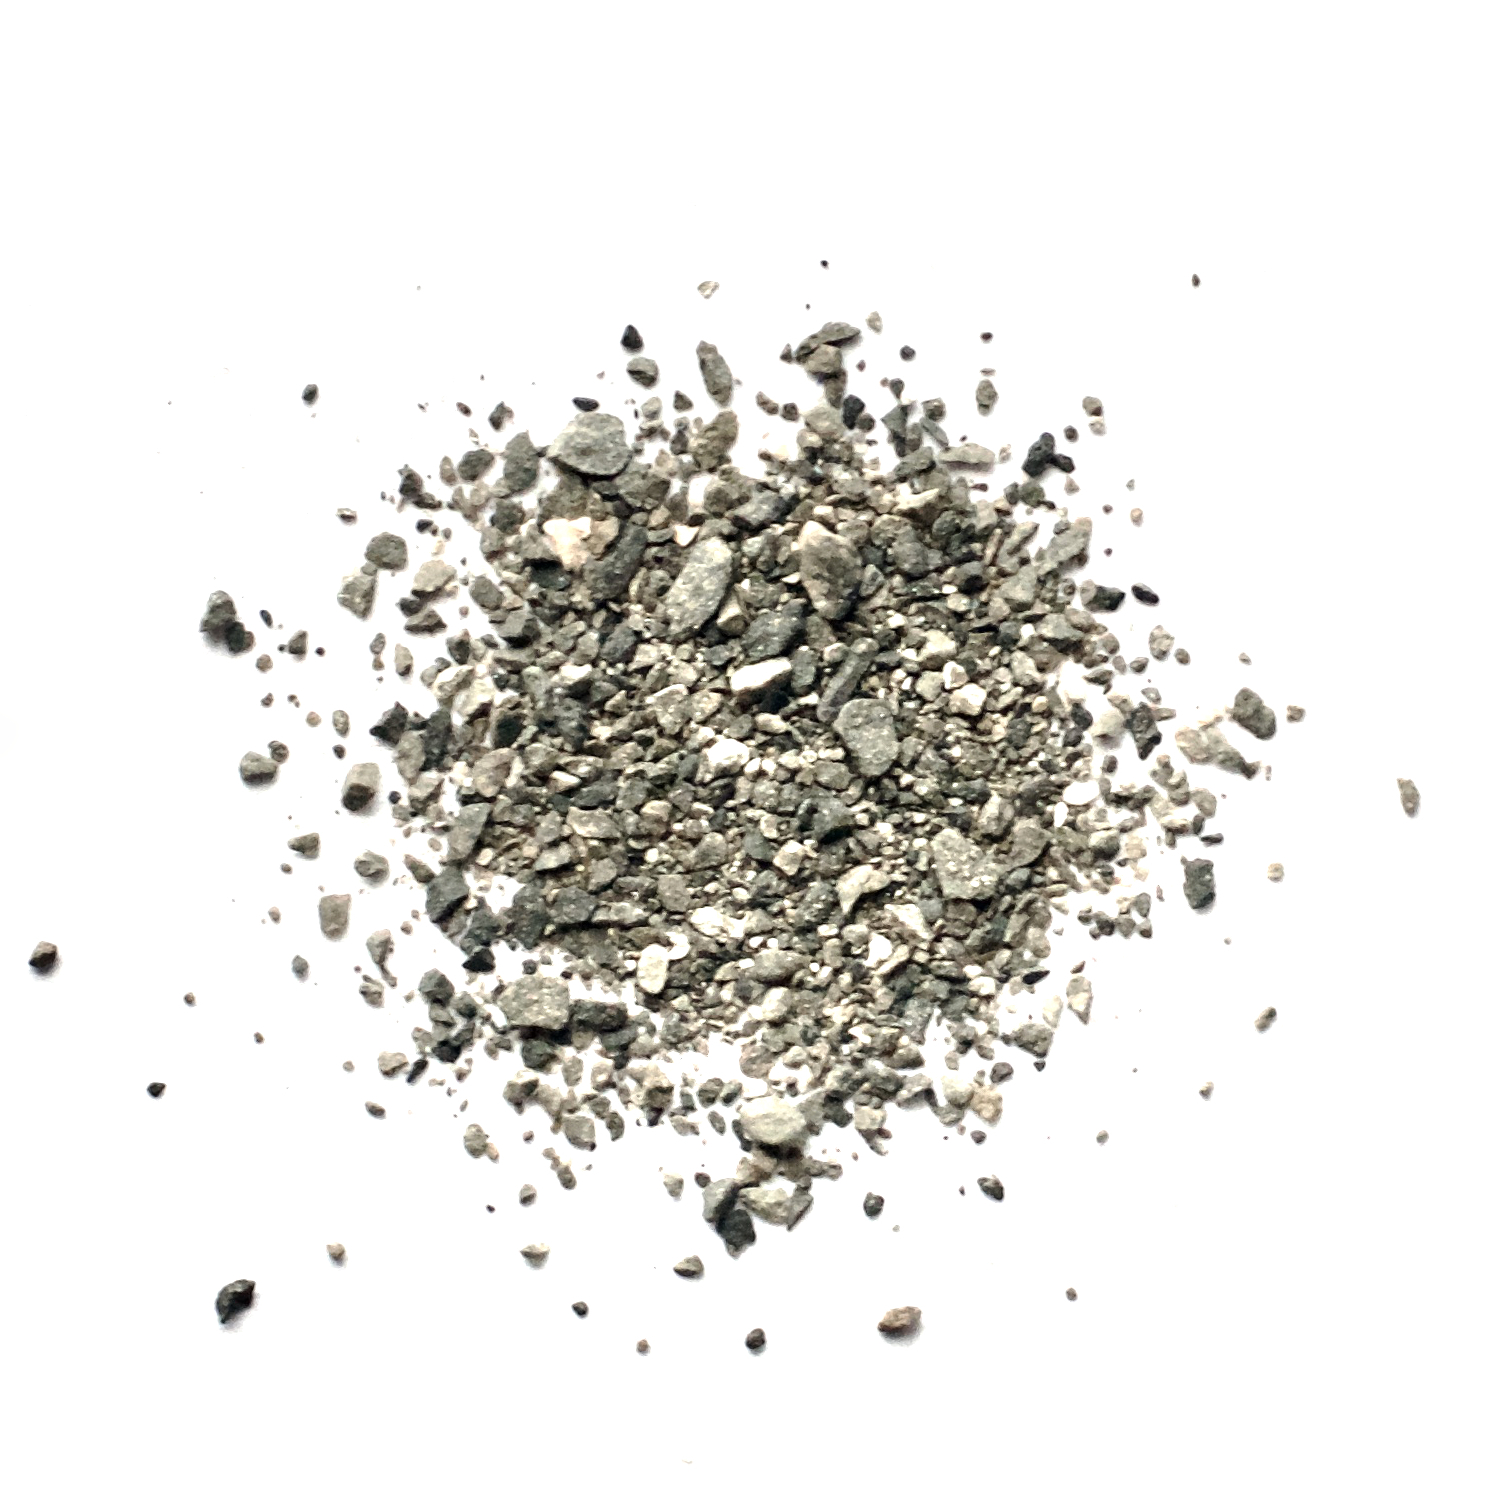
\includegraphics[width=\textwidth]{E5R}
		\caption{Ziarna rudy miedzi klasy E5R}
	\end{subfigure}
	\quad\quad
	\begin{subfigure}[t]{0.35\textwidth}
		\centering
		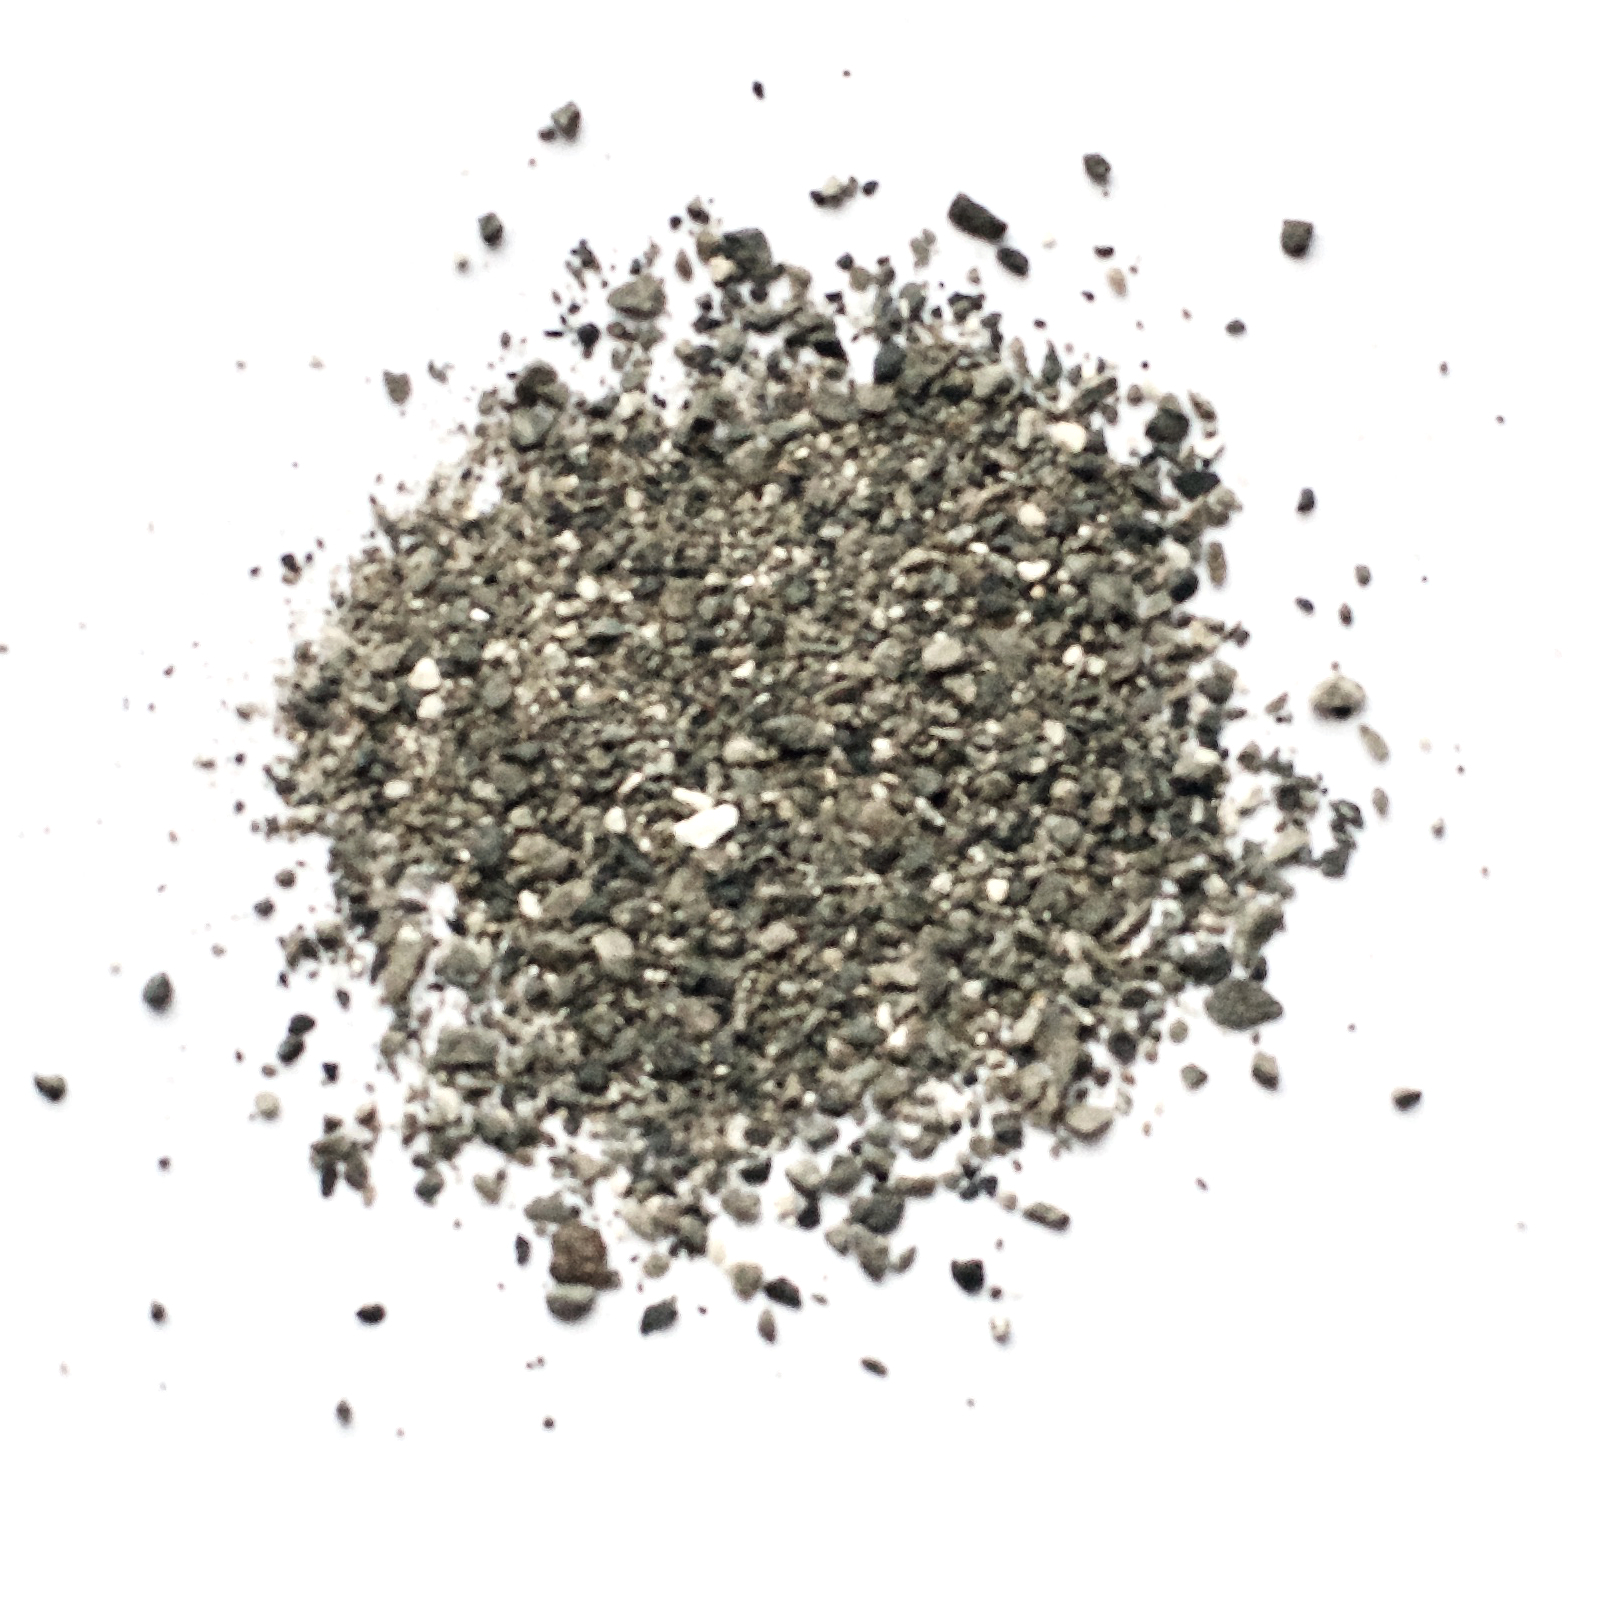
\includegraphics[width=\textwidth]{E6R}
		\caption{Ziarna rudy miedzi klasy E6R}
	\end{subfigure}
	\vskip\baselineskip
	\begin{subfigure}[t]{0.35\textwidth}
		\centering
		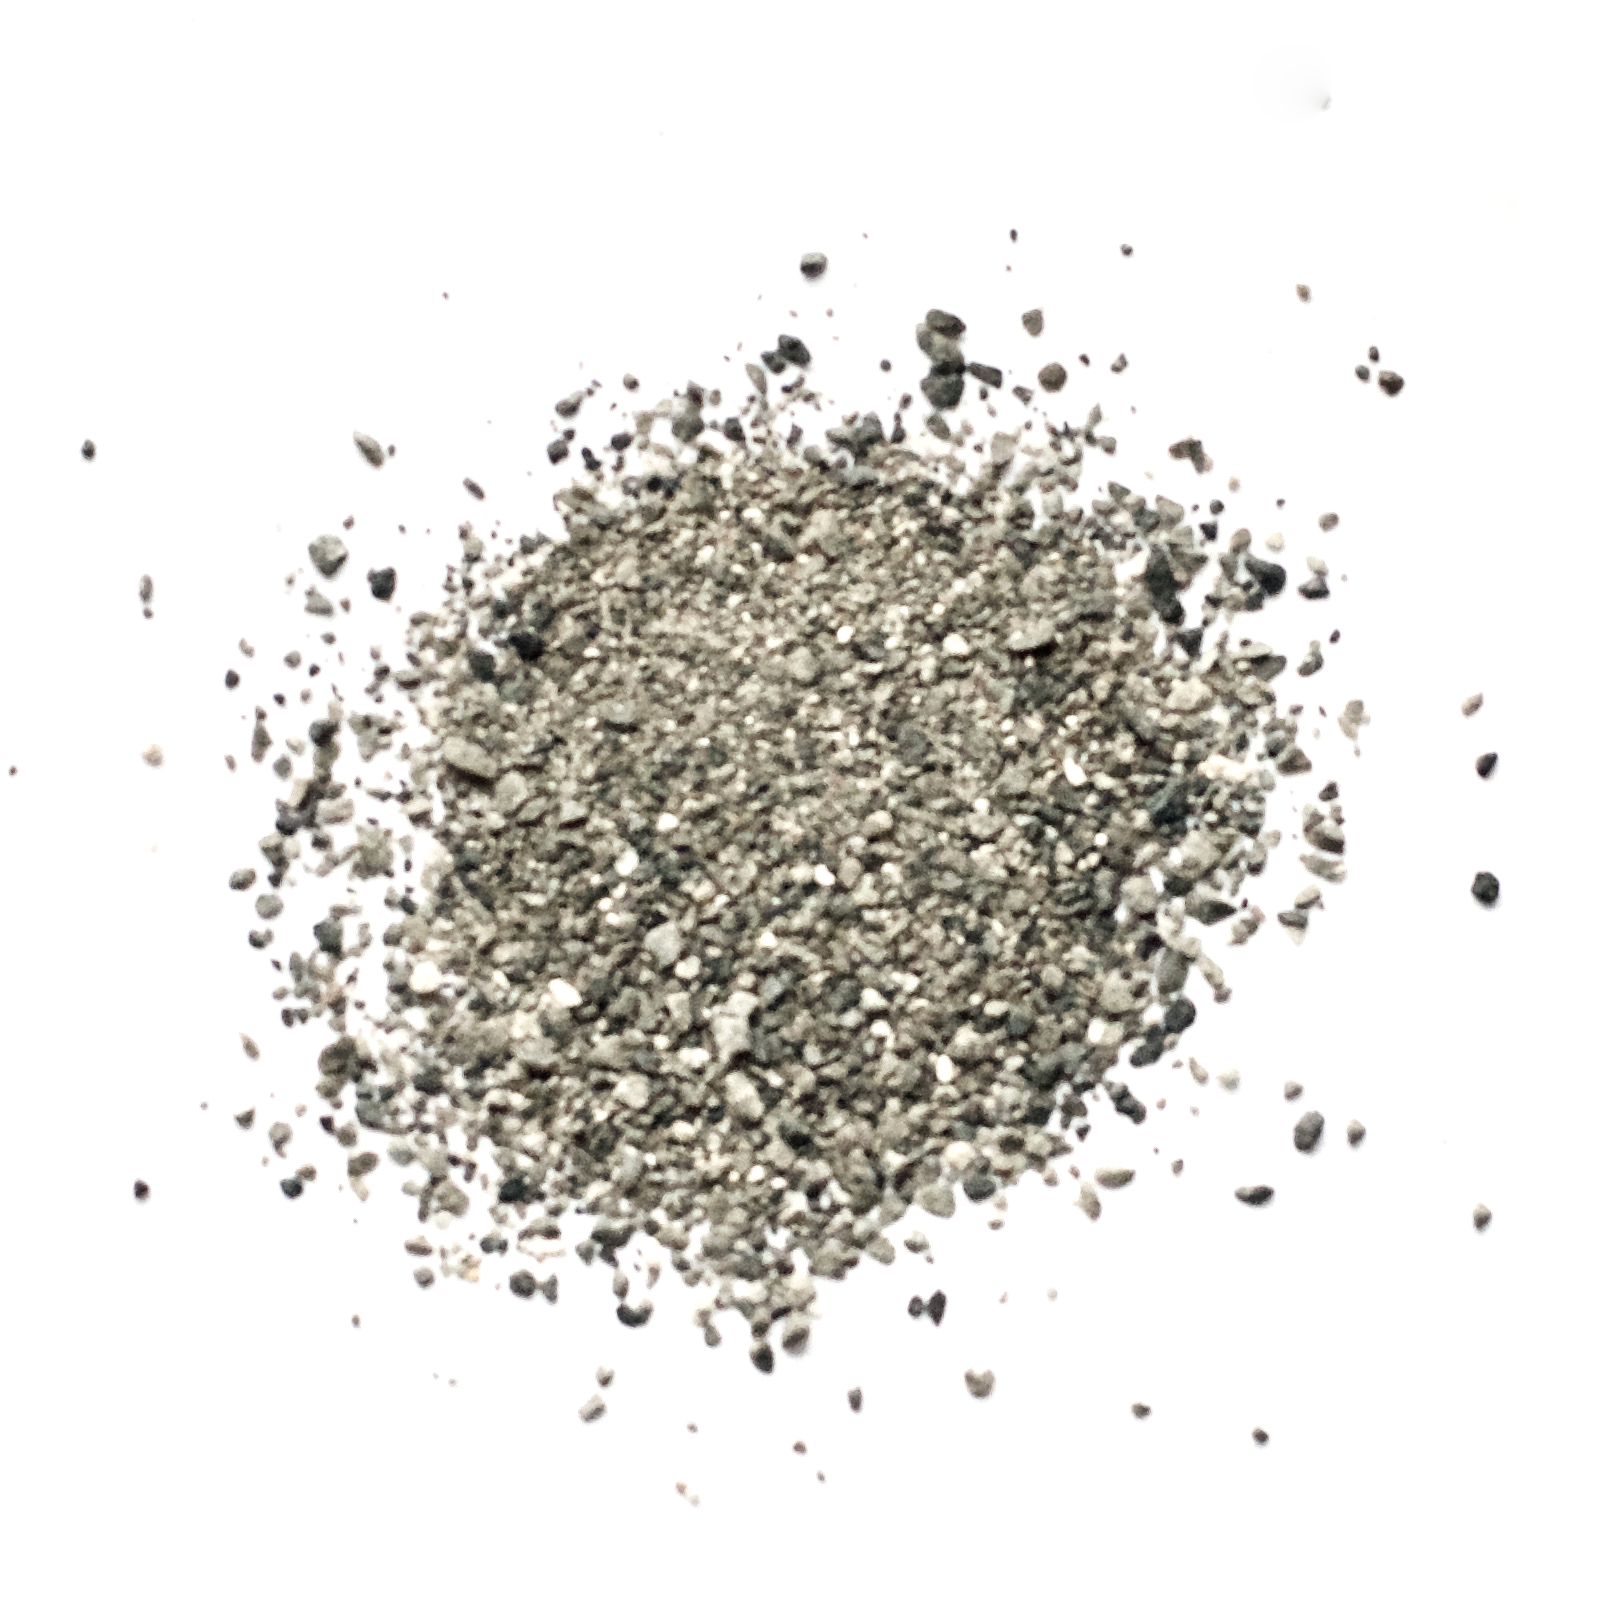
\includegraphics[width=\textwidth]{E11R}
		\caption{Ziarna rudy miedzi klasy E11R}
	\end{subfigure}
	\quad\quad
	\begin{subfigure}[t]{0.35\textwidth}
		\centering
		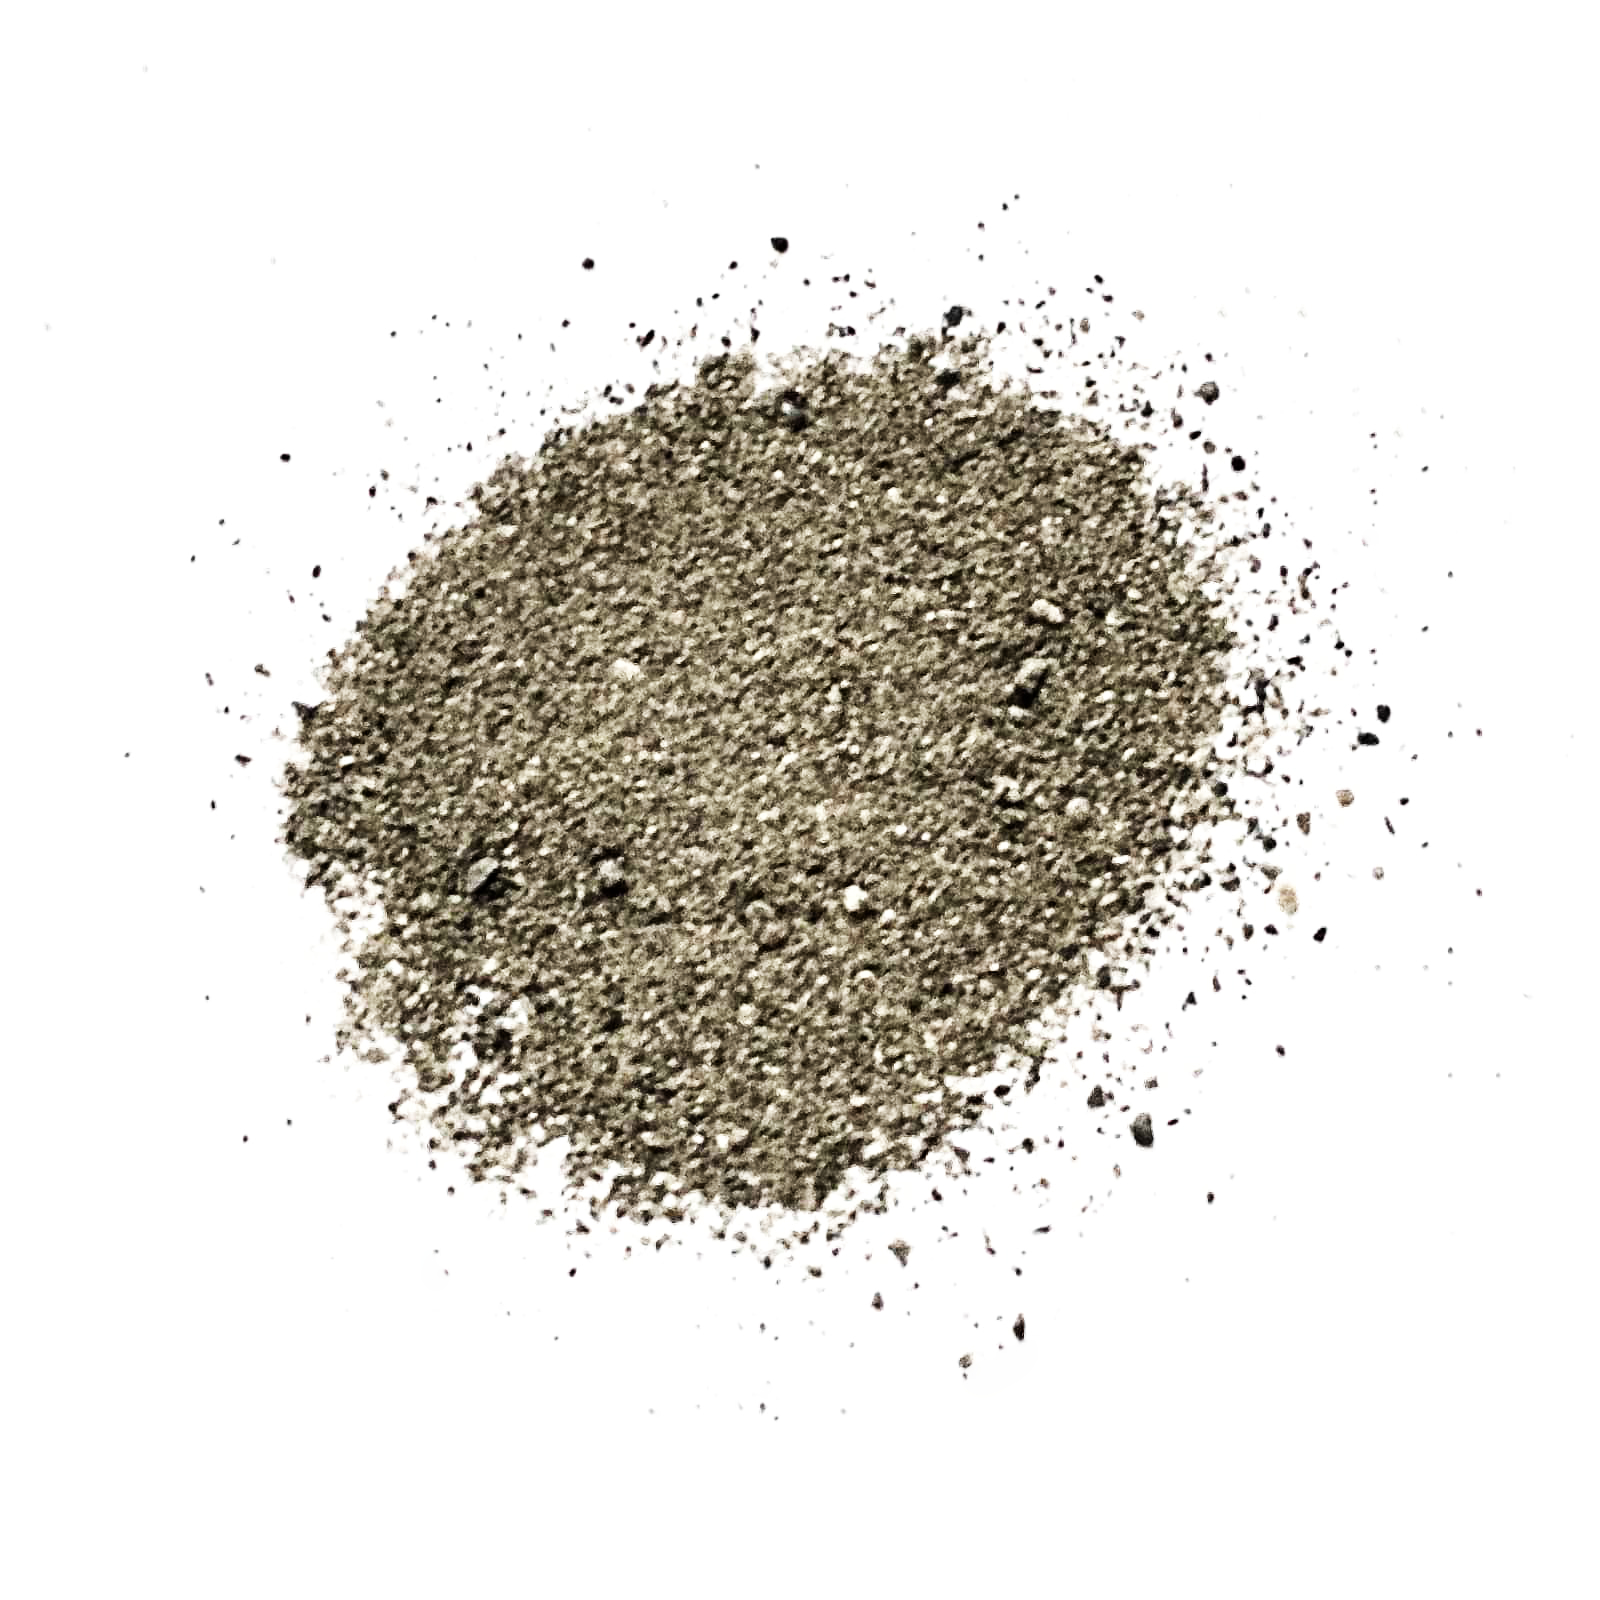
\includegraphics[width=\textwidth]{E16R}
		\caption{Ziarna rudy miedzi klasy E16R}
	\end{subfigure}
	\caption{Próbki rozpatrywanych ziaren rud miedzi}
	\label{fig:grains}
\end{figure}

\section{Rodzaje termowizji i~idea pomiarów termowizyjnych}
\label{sec:thermovision}
Pomiary termowizyjne polegają na rejestracji promieniowania cieplnego obiektów
w~celu ustalenia ich temperatury.
Badania z~wykorzystaniem termowizji można podzielić na dwie grupy:
\emph{termowizję pasywną} oraz \emph{termowizję aktywną}.

Technika pasywna polega na rejestracji obrazów obiektów bez ingerencji w~ich
temperaturę w~czasie trwania pomiarów.
Można w~ten sposób obserwować przepływ ciepła w~urządzeniach technicznych,
procesach przemysłowych oraz biologicznych.
W~rozważanym w~pracy przypadku technika ta nie ma jednak zastosowania.
W~warunkach pokojowych badany materiał ma w~całej swojej objętości podobną
temperaturę, co skutkuje obrazem równomiernego szumu w~rejestrowanym obrazie.

Bardziej zaawansowaną techniką są pomiary z~wykorzystaniem termowizji
aktywnej.
W tym trybie pomiarów badane obiekty ogrzewa się w~powtarzalnych warunkach, 
a~następnie rejestruje proces ich stygnięcia.
Podczas dostarczania ciepła do obiektu oraz jego oddawania na obrazach
termowizyjnych można zaobserwować strukturę badanego obiektu.
Przedmioty o~niejednorodnej i~złożonej budowie nagrzewają się oraz stygną
nierównomiernie, co jest rejestrowane przez kamery termowizyjne.
W~ten sposób można dostrzec cechy obiektu niewidoczne gołym okiem, takie
jak zmiany jego gęstości, składu oraz uszkodzenia struktury.
Termowizję aktywną stosuje się szeroko w~badaniach naukowych oraz przemyśle.
Przykładowe aplikacje tej techniki to detekcja defektów w~produktach
przemysłowych oraz wykrywanie części konstrukcji podatnych na zużycie.
Termowizja aktywna ma charakter niedestruktywny oraz bezkontaktowy,
co stanowi jej zalety w~analizie materiałowej \cite{ciampa_thermography}.
Technika ta wymaga jednak etapowego procesu pomiarowego, potrzebne jest 
przygotowanie instalacji grzewczej, a~nagrzewanie i~stygnięcie materiału
może być czasochłonne.
Przebieg zmian temperatury najlepiej rejestrować na materiałach wideo,
aby zmaksymalizować ilość danych zgromadzonych w~trakcie eksperymentu.

\section{Kamera termowizyjna FLIR A320}
\label{sec:camera}
Przedmiotem projektu jest analiza obrazów pochodzących z~przemysłowej
kamery termowizyjnej FLIR A320.
Firma FLIR zajmuje się produkcją wysokiej jakości kamer i~detektorów do celów
profesjonalnych i~przemysłowych.
Używany aparat łączy wysoką jakość pomiaru z~nowoczesnymi funkcjami
integracji z~oprogramowaniem komputerowym.
Urządzenie komunikuje się z~komputerem za pomocą sieci internetowej,
pozwalając na kontrolę z~poziomu aplikacji oraz bibliotek
programistycznych.
Dodatkowo kamera posiada możliwość planowania automatycznych pomiarów
i~alarmów, oferuje także funkcje analityczne oraz wbudowany serwer
internetowy \cite{flir_a32x_manual}.

\subsection{Opis sprzętowy wykorzystywanej kamery}
Kamera ma postać podłużnego korpusu, do którego swobodnie można podłączać
obiektywy.
Na rysunku \ref{fig:camera}~przedstawiono zdjęcie wykorzystywanego urządzenia.
\begin{figure}[htb]
    \centering
    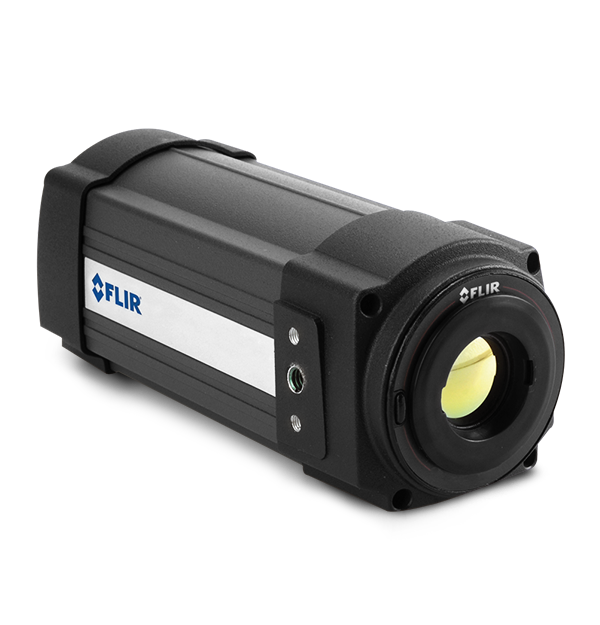
\includegraphics[width=0.5\textwidth]{flir_a320}
    \caption{Kamera termowizyjna FLIR A320 \cite{flir_camera_specs}}
    \label{fig:camera}
\end{figure}
Egzemplarz kamery znajdujący się w~laboratorium termowizji Politechniki
Śląskiej został wyposażony w~obiektyw, pozwalający oglądać ziarna rud miedzi
w~powiększeniu.
Kamera cechuje się następującymi parametrami \cite{flir_camera_specs}:
\begin{itemize}
	\item typ detektora: niechłodzony mikrobolometr
	\item rozdzielczość: 320 na 240 pikseli,
	\item częstotliwość odświeżania: \SI{9}{\hertz} do \SI{30}{\hertz}
	\item szerokość otworu: \textit{f}\num{1,3},
	\item autofokus z wbudowanym silnikiem,
	\item zakres pomiarowy temperatur: 
		\begin{enumerate}
			\item od \SI{-15}{\celsius} do \SI{+50}{\celsius},
			\item od \SI{0}{\celsius} do \SI{350}{\celsius},
		\end{enumerate}
	\item dokładność: \num{\pm2}\si{\celsius} lub \num{\pm2}\% odczytu,
	\item zakres wykrywanego widma promieniowania: \SI{7,5}{\micro\meter}
          do \SI{13}{\micro\meter}.
\end{itemize}

Kamera wykrywa temperaturę przez detektor zwany \emph{bolometrem},
który mierzy energię niesioną przez fale elektromagnetyczne w~spektrum
podczerwieni.
Kiedy fala pada na detektor aparatu, temperatura komórek matrycy rośnie
i~zwiększa się ich rezystancja elektryczna.
Wartości rezystancji są mierzone, a~na ich podstawie określana jest
temperatura \cite{vanhoof_infrared}.

Zakres temperatur kamery jest odpowiedni do przeprowadzenia eksperymentów
z~pomiarami ziaren rud miedzi metodą termowizji aktywnej.
Próbki planuje się podgrzewać do temperatury maksymalnie około
\SI{80}{\celsius},~wartość ta mieści się w~zakresie pracy urządzenia.
Dokładność kamery jest zadowalająca, próbne materiały nagraniowe
wskazały, że na zdjęciach widocznych jest wiele szczegółów i~detali
badanego materiału.
Przy klasyfikacji obrazów i~wzorców stygnięcia próbek jest to 
bardziej istotne niż liczbowa dokładność pomiarowa przyrządu.

W~porównaniu ze zwykłymi, współczesnymi aparatami, rozdzielczość kamery
termowizyjnej może wydawać się mała.
Należy sobie jednak uzmysłowić, że w~standardowych aparatach piksele mają
rozkład Bayera, a~wartości składowych koloru są interpolowane.
W~kamerze termowizyjnej każda komórka matrycy dokonuje pełnego pomiaru
wartości temperatury.
Z~tego powodu bezpośrednie porównanie rozdzielczości używanego
przyrządu z~popularnymi aparatami może być mylące.
Oczywiście większa rozdzielczość kamery byłaby pożądana, jednak jej obecne
możliwości pozwalają na szczegółowe pomiary i~obserwację wielu detali ziaren
rud miedzi.

\subsection{Obiektyw kamery}
\label{subsec:lens}
Kamerę wyposażono w~obiektyw zbliżeniowy FLIR~T197415, pozwalający obserwować
ziarna rud miedzy.
Jest to sprzęt zaprojektowany przez producentów używanej kamery i~dedykowany
pracy z~urządzeniami termowizyjnymi.
Przyrząd przedstawiono na rysunku \ref{fig:lens}.
\begin{figure}[htb]
    \centering
    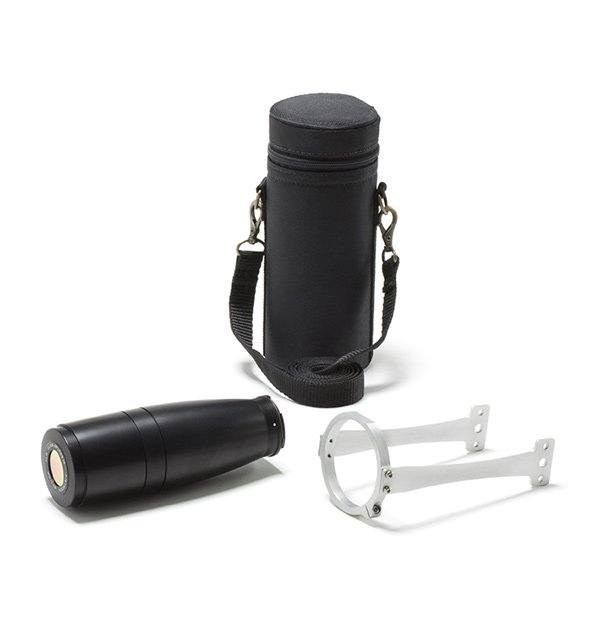
\includegraphics[width=0.5\textwidth]{flir_lens}
    \caption{Obiektyw FLIR T197415 \cite{flir_lens_specs}}
    \label{fig:lens}
\end{figure}
Wybrany obiektyw jest przygotowany z~myślą o~obserwacji drobnych detali
powierzchni w~dużym zbliżeniu.
Używany model ma następujące parametry \cite{flir_lens_specs}:
\begin{itemize}
	\item ogniskowa: \SI{18,2}{\milli\meter},
	\item powiększenie: \num{1x1},
	\item pole widzenia: \SI{8}{\milli\meter} na \SI{6}{\milli\meter},
	\item odległość od płaszczyzny ostrzenia: \SI{20}{\milli\meter},
	\item głębia ostrości: \SI{0,3}{\milli\meter},
	\item przysłona: bez regulacji, równa otworowi systemu montażu kamery,
	\item budowa: trzy soczewki asferyczne.
\end{itemize}

Zgodnie ze specyfikacją producenta obiektyw ma powiększenie \num{1x1},~co
może wydawać się niedużą wartością.
Należy mieć jednak świadomość, że zwykłe obiektywy zmniejszają obraz
padający na matrycę.
Powszechnie  jako granicę makrofotografii przyjmuje się
powiększenie \num{1x1}.~
W~obserwacji ziaren i~detali powierzchni nie jest jednak istotne powiększenie,
ale to że używany obiektyw jest \emph{zbliżeniowy}.
Oznacza to, że ma on bardzo małą odległość ostrzenia, czyli można go przysunąć
blisko obserwowanej powierzchni.
Obiektyw zbliżeniowy pozwala na obserwację z~dystansu
\SI{20}{\milli\meter},~typowe obiektywy ostrzą z~odległości parudziesięciu
centymetrów do ponad metra.
Dzięki temu obiektyw zbliżeniowy pozwala na obserwację bardzo drobnych
detali powierzchni.

\subsection{Oprogramowanie do obsługi kamery}
\label{subsec:camera_soft}
Jedną z~najważniejszych cech kamery jest łatwość integracji
z~oprogramowaniem komputerowym.
Kamerę można obsługiwać za pomocą programu FLIR Tools\footnote{Strona produktu
programu FLIR Tools: \url{https://www.flir.com/products/flir-tools/}}.
Pozwala on na podgląd obrazu oraz wykonywanie zdjęć termowizyjnych.
Producent dostarcza również bibliotekę LabVIEW pozwalającą na zaawansowaną
pracę z~kamerą.
Do obsługi stanowiska został napisany program używający tych bibliotek,
który pozwala na nagrywanie materiałów wideo przy pomocy kamery.
Nagrania mają własnościowy format firmy FLIR, można je odtwarzać w~programie
FLIR Tools.
Program pozwala także na eksport stopklatek z~nagrania w~postaci plików JPEG.
Przy obsłudze narzędzia ważne jest ustawianie zakresu temperatur na obrazie.
Wybrany zakres określa w~jaki sposób wartości temperatury są mapowane na
kolory na zdjęciu, zawarte w~tablicy LUT.
Program oferuje tablice w~skali szarości, takie zostały użyte w~projekcie,
możliwy jest także wybór tablic w~postaci kolorowych gradientów.
Wybór zakresu wpływa na wygląd wyświetlanego obrazu oraz eksportowanych
stopklatek.
Jego nieodpowiedni dobór może skutkować zbyt ciemnym, jasnym, lub mało
kontrastowym obrazem.
Aby zapewnić najlepsze wykorzystanie nagrań z~kamery oraz powtarzalny
charakter eksportu stopklatek korzystano z~opcji automatycznego doboru
zakresu temperatur, jaki jest wbudowany w~program FLIR Tools.

\section{Narzędzia programistyczne}

\subsection{Język programowania Python}
Założenia projektu wymagają użycia języka programowania pozwalającego
na zaawansowaną obróbkę obrazu oraz wydajne budowanie sieci neuronowych.
W~obu tych dziedzinach wiodącym językiem jest Python, posiadający bogaty
zestaw bibliotek.
Język ten oferuje dużą wygodę programowania, co jest istotne przy pracy 
badawczej.
Jednocześnie Python jest zaopatrzony w~wydajną bibliotekę obliczeń
numerycznych NumPy.
Oferuje ona klasy macierzy numerycznych oraz bogaty zestaw operacji
matematycznych.
Macierze biblioteki NumPy są mniej elastyczne od zwykłych list języka Python,
jednak oferują dużo większą wydajność obliczeniową, między innymi dzięki
wsparciu obliczeń wektorowych na odpowiednich procesorach.
Wiele innych bibliotek języka wykorzystuje pakiet NumPy, na przykład przy
przetwarzaniu obrazów, co pozwala na wysoką wydajność obliczeń.
Połączenie wygody programowania z~zadowalającą wydajnością bibliotek
numerycznych, sprawia że Python jest dobrym wyborem do realizacji
założeń projektu.

\subsection{Biblioteka przetwarzania obrazu Scikit-image}
Język Python oferuje bogaty zestaw bibliotek przetwarzania obrazu.
Najbardziej popularną z~nich jest biblioteka OpenCV napisana w~języku
C\texttt{++}.
Zdecydowano się jednak na wybór mniej znanego pakietu Scikit-image.
Jest to biblioteka zorientowana na obliczenia naukowe i~badawcze
oraz napisana bezpośrednio z~myślą o~języku Python \cite{scikit-image}.
Scikit-image, w~porównaniu z OpenCV, oferuje bardziej spójny interfejs
programisty oraz lepiej wykorzystuje charakterystykę języka Python.
Dodatkowo wybrana biblioteka jest częścią zestawu Scikit, w~skład
którego wchodzi pakiet Scikit-learn służący do uczenia maszynowego.
Może on być przydatny przy tworzeniu sieci neuronowej, a~spójność bibliotek
z~pakietu Scikit jest niewątpliwie zaletą.
Wybrana biblioteka charakteryzuje się również dobrą dokumentacją
\cite{scikit_reference} oraz zestawem przykładów.

\subsection{Interfejs sieci neuronowych Keras}
\label{subsec:software_network}
Wybór bibliotek głębokiego uczenia w~języku Python jest bardzo szeroki.
Do najpopularniejszych pakietów należą: Keras, TensorFlow oraz PyTorch.
Zdecydowano się na wybór interfejsu biblioteki Keras.
Jest to pakiet nastawiony na elastyczność i~możliwość eksperymentowania,
oferuje wysokopoziomową, matematyczną warstwę abstrakcji opisu sieci
neuronowych \cite{chollet_keras}.
Moduł Keras oferuje także rozbudowaną dokumentację oraz zestaw poradników
\cite{keras_docs}.
Keras nie jest jednak pełnym rozwiązaniem, a~raczej abstrakcyjnym interfejsem.
Używanie go wymaga wyboru wewnętrznego silnika biblioteki.
Zdecydowano się na domyślną opcję użycia zaplecza pakietu TensorFlow.
W~standardowy sposób interfejsu Keras używa się po osobnym zainstalowaniu
jego modułów i~wskazaniu silnika sieci neuronowych.
Biblioteka TensorFlow udostępnia jednak wewnętrzny interfejs Keras,
co pozwala na zwiększenie wydajności obliczeniowej w~połączeniu dwóch
bibliotek.
Przy tworzeniu oprogramowania wzięto to pod uwagę i~użyto bardziej wydajnej
metody importowania interfejsu Keras.


\chapter{Analiza i~ekstrakcja danych termowizyjnych}
\section{Proces pomiarowy i~budowa zbioru danych}
\label{sec:measure}
Zgodnie z~opisem technik termowizyjnych przedstawionym w~sekcji
\ref{sec:thermovision}~zdecydowano się na przeprowadzenie pomiarów za pomocą
termowizji aktywnej.
Aby zrealizować pomiary przygotowano stanowisko laboratoryjne.
Kamera termowizyjna została umieszczona na statywie, a~do ogrzewania próbek
zdecydowano się wykorzystać lampę halogenową.

W~procesie termowizji aktywnej istotny jest charakter procesu nagrzewania
materiału.
Przy przygotowaniu pomiarów należy zdecydować pod jakim warunkiem zakończyć
przekazywanie ciepła do próbki.
Rozważono dwie możliwości:
\begin{enumerate}[a)]
    \item ogrzewanie próbek do osiągnięcia ustalonej temperatury,
    \item \label{it:heat_method}
          ogrzewanie próbek przez ustalony czas.
\end{enumerate}
Zdecydowano się na metodę \ref{it:heat_method},~ze względu na wygodę jej
realizacji.
Doprowadzenie każdej próbki do tej samej temperatury wymaga pomiarów w~czasie
nagrzewania, co jest bardziej wymagające w~realizacji.
Wstępne obserwacje nagrań wskazują, że nagrzewanie materiału przez ustalony
czas, pozwala na obserwacje unikalnych wzorców stygnięcia ziaren.

Następnie wybrano czas nagrywania materiałów wideo.
Na podstawie próbnych nagrań zdecydowano się na ogrzewanie próbek przez jedną
minutę oraz rejestrację ich stygnięcia przez cztery minuty.
Taka konfiguracja daje, przy badanych pyłach rud miedzi, ostry i~szczegółowy
obraz w~początkowej fazie nagrywania oraz widocznie rozmazany i~mniej
kontrastowy materiał pod koniec stygnięcia.
Charakter procesu przejścia między tymi stanami pozwoli na klasyfikację badanych
ziaren rud miedzi.

Ostatnia decyzja kształtująca charakter pomiarów dotyczy chwili przechwytywania
stopklatek z~pozyskanych materiałów wideo.
Na podstawie obserwacji zdecydowano się eksportować pięć klatek, jedną na
początku każdej minuty nagrania.

Po ustaleniu planu eksperymentu pomiarowego przystąpiono do jego wykonania.
Zgodnie z~opisem badanych materiałów w~sekcji \ref{sec:grains},~zgromadzono
nagrania wideo dla czterech klas ziaren rudy miedzi.
Ze względu na czasochłonność pomiarów dla każdej klasy materiału nagrano trzy
filmy.
Przy nagrywaniu stygnięcia tej samej klasy materiału pomiędzy pomiarami próbkę
poddawano przemieszaniu, aby uniknąć powtarzania struktur ułożenia ziaren.
Zgodnie z~opisem w~podsekcji \ref{subsec:camera_soft},~podczas zapisu zdjęć,
używano opcji automatycznego doboru zakresu temperatur.

Proces pomiarowy w~protypowych warunkach był obarczony brakiem dużej precyzji
i~powtarzalności.
Obserwacja uzyskanych nagrań pokazała, że obrazy tej samej klasy ziaren
niekoniecznie osiągały równą temperaturę po ogrzewaniu przez ustalony czas.
Problemem okazało się również dostosowanie ostrości obrazu z~kamery.
Jak wytłumaczono w~podsekcji \ref{subsec:lens}~wykorzystywany aparat cechuje
się bardzo małą głębią ostrości, co powoduje że drobne ruchy kamery mogą
spowodować utratę czytelności obrazu.
Z~kolei proces pomiarowy wymagał ciągłego przenoszenia próbki między
stanowiskiem do podgrzewania materiału oraz nagrywania filmów.
Należy mieć na uwadze że w~czasie układania próbek pod kamerą oraz poprawiania
ostrości postępowało stygnięcie ziaren, co sprzyjało brakowi powtarzalności
pomiarów.
Ze względu na przypadkowe utraty ostrości przy nagrywaniu oraz zbyt długi czas
przenoszenia i~przygotowania próbki do nagrywania, eksperyment wymagał czasem
powtarzania.
Ostatecznie jakość procesu pomiarowego oceniono na podstawie jego wyników
w~klasyfikacji ziaren, po skonstruowaniu sieci neuronowej.

\section{Analiza obrazów termowizyjnych}
Zgodnie z~zamysłem pomiarów przedstawionym w~sekcji \ref{sec:measure}~z~każdego
nagrania wybrano pięć stopklatek.
Podczas eksperymentu uzyskano łącznie dwanaście pomiarów, zawierających
sumarycznie 60~zdjęć.
W~ramach uczenia maszynowego jest to bardzo mały zbiór danych, biorąc jednak
pod uwagę wstępno-badawczy charakter pracy oraz czasochłonność procesu
pomiarowego zdecydowano, że jest to rozmiar zadawalający do pierwszych prób
klasyfikacji.
Zebrane materiały mają format JPEG, do oznaczania zdjęć przyjęto schemat nazw
jak w~przykładzie: 115\_E11R\_1, gdzie człony nazwy oznaczają kolejno:
\begin{itemize}
    \item automatyczny numer nagrania w~programie FLIR Tools,
    \item klasę próbki,
    \item minutę nagrania.
\end{itemize}

\subsection{Prezentacja przykładowej serii pomiarowej}
Jak opisano w rozdziale \ref{sec:measure}~jedna próbka w~zbiorze danych składa
się z~serii pięciu zdjęć o~malejącym kontraście i~szczegółowości.
Na rysunku \ref{fig:sample}~przedstawiono proces stygnięcia przykładowej
próbki 104~klasy E5R.
Wartości zakresu temperatur na zdjęciach maleją.
Wskazuje to na stopniowy spadek sumarycznej temperatury obserwowanego materiału.
Dodatkowo obraz staje się coraz mniej wyraźny i~kontrastowy.
Nagrzana próbka emituje ciepło ze swoich zróżnicowanych struktur w~niejednorodny
sposób.
Wraz z~ochłodzeniem ziaren temperatura na obrazie wyrównuje się i~kamera
termowizyjna rejestruje coraz mniej szczegółów.
Detale i~elementy charakterystyczne obrazu zlewają się na kolejnych zdjęciach.
Wraz z~opadaniem temperatury na zdjęciu pojawia się także coraz więcej szumów.
\begin{figure}[htbp]
    \centering
    \begin{subfigure}{0.45\textwidth}
        \centering
        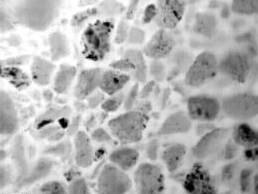
\includegraphics[width=\textwidth]{sample/104_E5R_0}
        \caption{Minuta: 0 \\
            Zakres temperatur: \SI{48.0}{\celsius} do
            \SI{53.0}{\celsius}}
    \end{subfigure}
    \hspace{0.75cm}
    \vspace{0.5cm}
    \begin{subfigure}{0.45\textwidth}
        \centering
        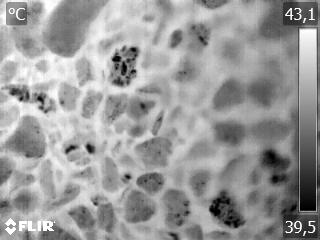
\includegraphics[width=\textwidth]{sample/104_E5R_1}
        \caption{Minuta: 1 \\
            Zakres temperatur: \SI{43.1}{\celsius} do
            \SI{39.5}{\celsius}}
    \end{subfigure}
    \begin{subfigure}{0.45\textwidth}
        \centering
        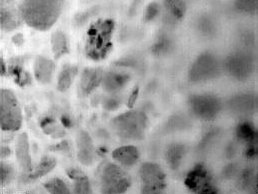
\includegraphics[width=\textwidth]{sample/104_E5R_2}
        \caption{Minuta: 2 \\
            Zakres temperatur: \SI{36.8}{\celsius} do
            \SI{39.5}{\celsius}}
    \end{subfigure}
    \hspace{0.75cm}
    \vspace{0.5cm}
    \begin{subfigure}{0.45\textwidth}
        \centering
        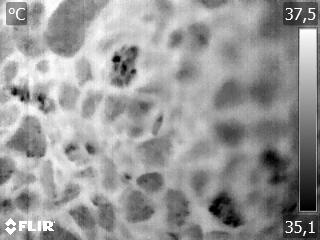
\includegraphics[width=\textwidth]{sample/104_E5R_3}
        \caption{Minuta: 3 \\
            Zakres temperatur: \SI{35.1}{\celsius} do
            \SI{37.5}{\celsius}}
    \end{subfigure}
    \begin{subfigure}{0.45\textwidth}
        \centering
        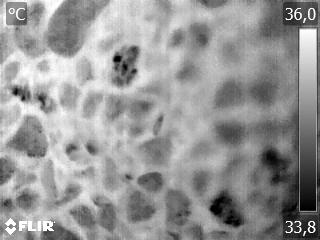
\includegraphics[width=\textwidth]{sample/104_E5R_4}
        \caption{Minuta: 4 \\
            Zakres temperatur: \SI{33.8}{\celsius} do
            \SI{36.8}{\celsius}}
    \end{subfigure}
    \caption{Zdjęcia procesu stygnięcia przykładowej próbki 104 klasy E5R}
    \label{fig:sample}
\end{figure}

\subsection{Przetwarzanie danych wizyjnych}
Wykorzystanie wizji komputerowej w~rozmaitych zadaniach często wymaga
odpowiedniego przygotowania używanych obrazów.
Do standardowych technik należą: wyrównywanie histogramu oraz redukcja szumów
i~wyostrzanie zdjęć.
Po analizie zebranych obrazów i~wypróbowaniu wymienionych technik zdecydowano
się jednak nie modyfikować zgromadzonych nagrań.
Użyty podczas pomiarów program FLIR Tools posiada wbudowaną funkcję doboru
zakresu temperatur, co przekłada się na ekspozycję i~kontrast eksportowanych
zdjęć.
Próba wyrównywania histogramu oraz korekcji kontrastu sprawiłaby, że obraz
rozkładu temperatur na zdjęciu stałby się przekłamany.
Ze względu na niską, jak na standardy typowego przetwarzania zdjęć cyfrowych,
rozdzielczość obrazów zrezygnowano także z~redukcji szumów.
Wiele detali ziaren ma wielkość zaledwie paru pikseli, proces usuwania szumu
mógłby spowodować ich zanik.
Nie oznacza to jednak, że zdjęcia charakteryzują się przypadkową ekspozycją.
Algorytmy automatycznego doboru zakresu temperatur kamery dbają o~to, by obraz
oddawał właściwości cieplne obiektu.

\subsection{Odczyt zakresu pomiarowego temperatur z~obrazu}
Jak wspomniano w~sekcji \ref{subsec:camera_soft}~jednym z~kluczowych czynników
decydujących o~wyglądzie obrazów pochodzących z~kamery jest zakres temperatur
mapowany na kolory w~obrazie.
Niestety aplikacja FLIR Tools nie pozwala na eksport zakresu temperatur wraz ze
zdjęciami w~formacie liczbowym.
W~czasie zapisu zdjęć oprogramowanie dodaje do nich interfejs z~aktywną skalą
pomiarową, jednak jest on graficznie naniesiony na obraz.
Aby ułatwić w~przyszłości pracę z~materiałami z~kamery opracowano mechanizm
ekstrakcji zakresu temperatur z~zdjęć pochodzących z kamery.

W~celu odczytu wartości liczbowych z~obrazu posłużono się gotową siecią
neuronową zaprojektowaną do detekcji tekstu na zdjęciach.
Zdecydowano się na użycie popularnej biblioteki \emph{Pytesseract}
\footnote{%
    Repozytorium projektu w~serwisie GitHub:
    \url{https://github.com/madmaze/pytesseract}}.
Analizowane zdjęcia są kadrowane, by wyizolować odczytywane liczby.
Wycięte fragmenty mają bardzo małą rozdzielczość, aby ułatwić sieci
rozpoznawanie liczb, zdecydowano się przeskalować obrazy w~górę.
W~czasie skalowania włączono mechanizm anty aliasingu aby wyrównać krawędzie
cyfr.
Ponieważ używana sieć uznaje za tło kolor biały oraz poszukuje liczb w~kolorze
czarnym, barwy na zdjęciu odwrócono.
Następnie obraz poddano binaryzacji metodą \emph{otsu}.
Jest to popularna i~wydajna metoda binaryzacji, jej efektywność jest maksymalna
kiedy liczba pikseli tła oraz pierwszego planu jest zbliżona
\cite{sezgin_thresholding}.
Z~tego powodu poprawne kadrowanie liczb sprzyja jakości ich binaryzacji.
Na rysunku \ref{fig:temp_bounds}~przedstawiono kolejne etapy przygotowania
obrazu do rozpoznania liczb.
Implementację opisanego mechanizmu odczytywania zakresu temperatur ze zdjęć
przedstawiono na listingu \ref{lst:temp_bounds}.
\begin{figure}[htbp]
    \centering
    \begin{subfigure}{0.45\textwidth}
        \centering
        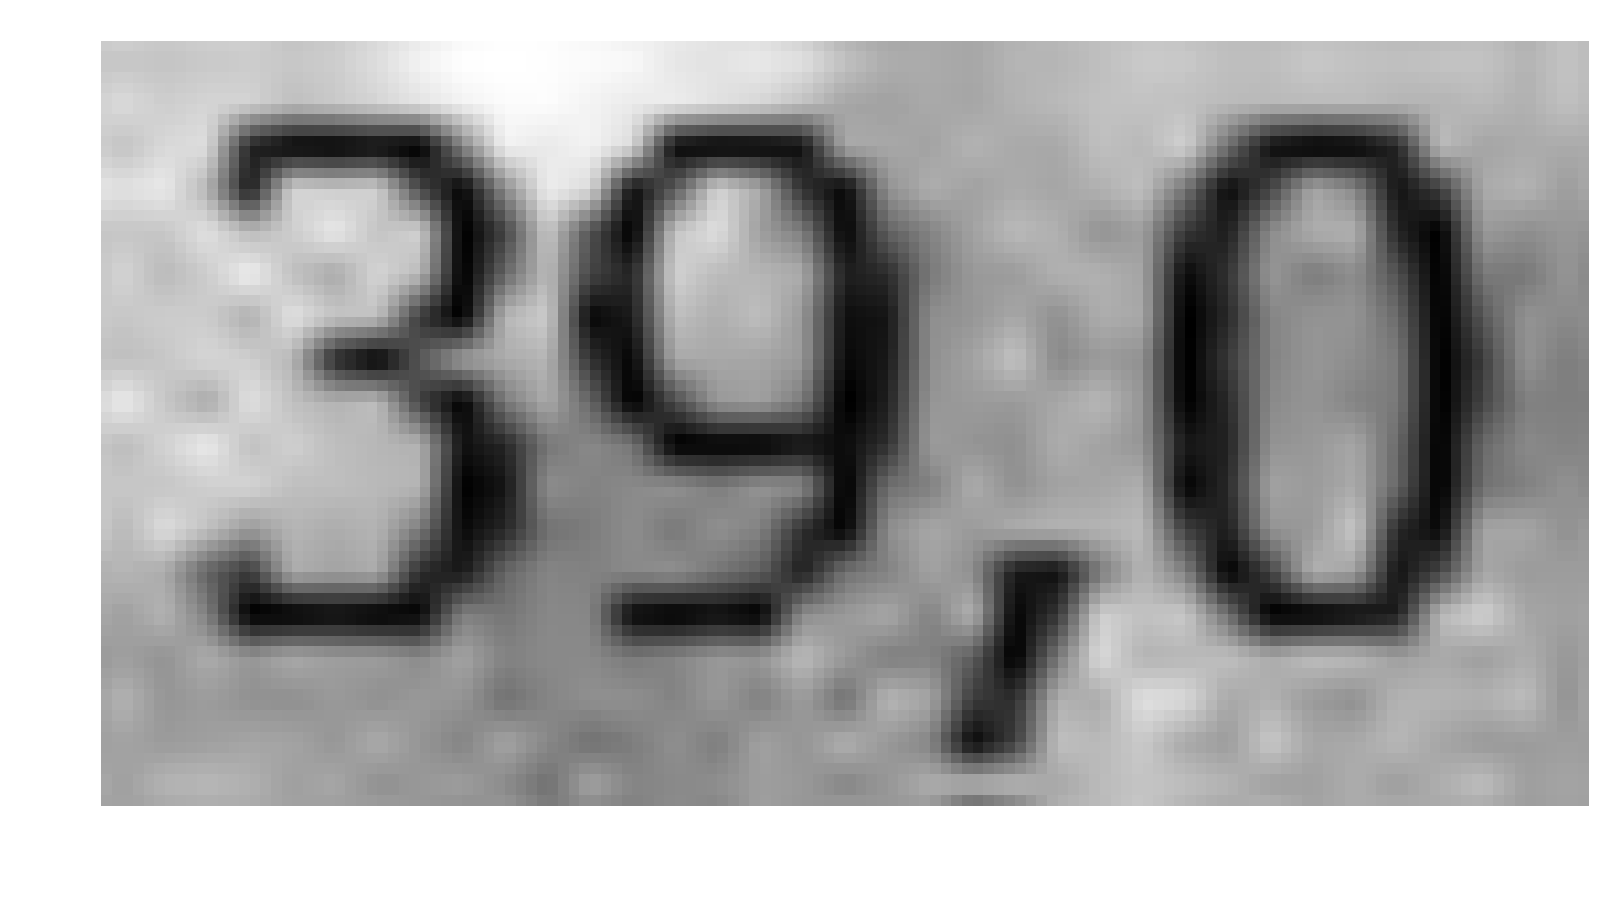
\includegraphics[width=\textwidth]{temp_bounds_scale}
        \caption{Przeskalowany kadr z~liczbą}
        \label{fig:temp_bounds_scale}
    \end{subfigure}
    \hspace{0.5cm}
    \begin{subfigure}{0.45\textwidth}
        \centering
        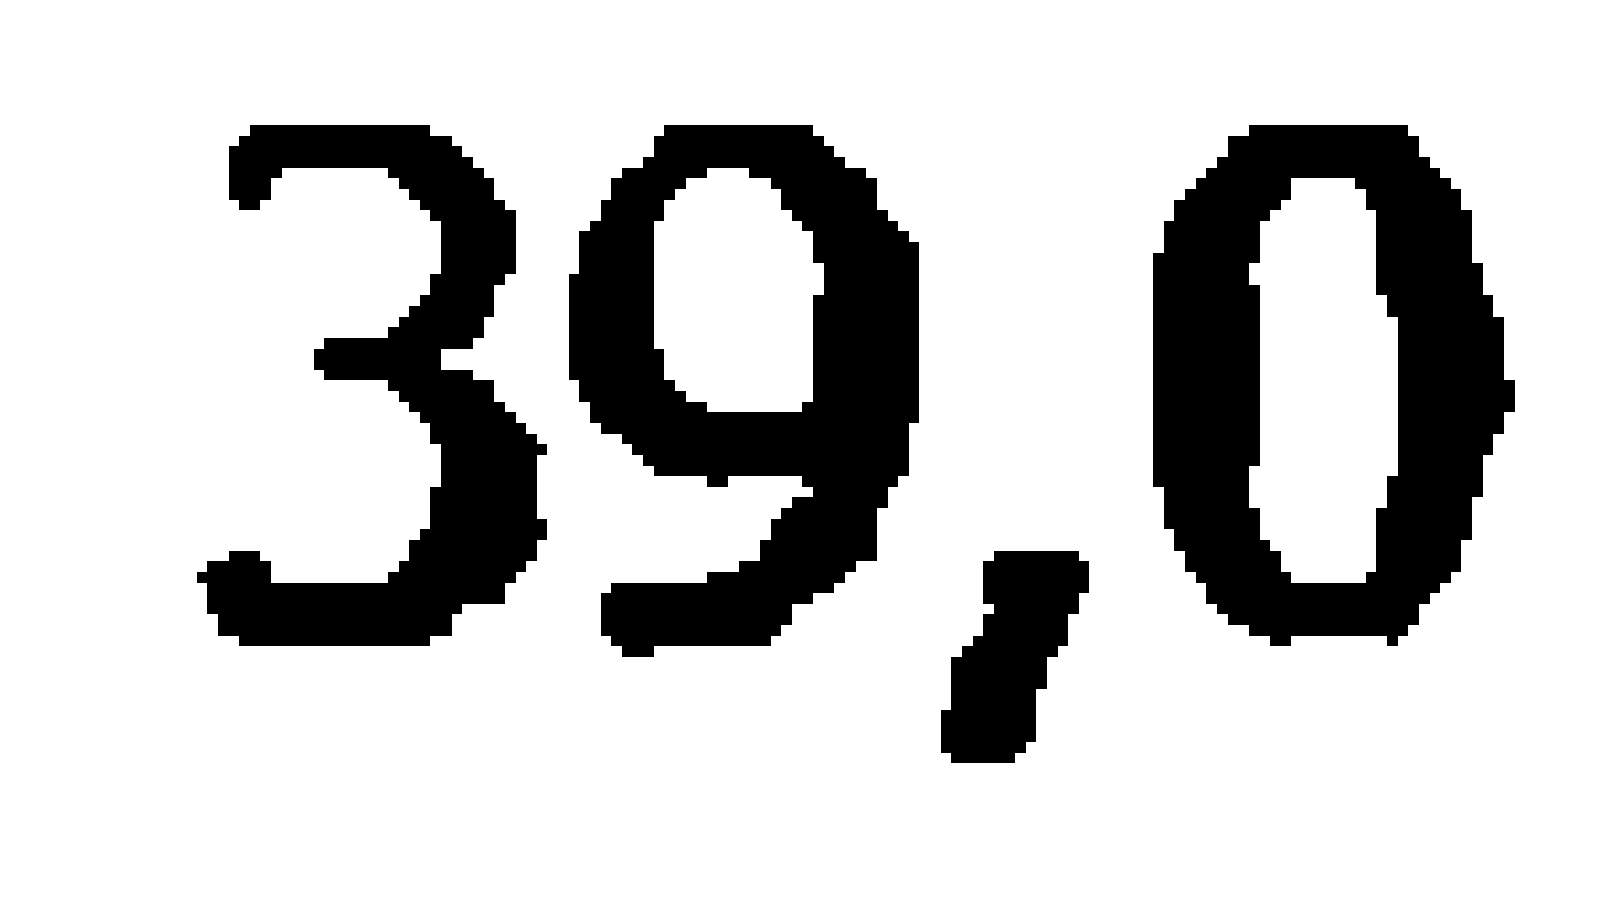
\includegraphics[width=\textwidth]{temp_bounds_bin}
        \caption{Kadr z~liczbą po binaryzacji}
        \label{fig:temp_bounds_bin}
    \end{subfigure}
    \caption{Przygotowanie zakresu temperatur do odczytu przez sieć neuronową}
    \label{fig:temp_bounds}
\end{figure}

\begin{listing}[htbp]
\begin{minted}{python}
def get_temperature_bounds(img, bounds=(((6, 24), (283, 318)),
                                        ((219, 236), (283, 318)))):
    '''Extract temperature values from FLIR UI on image.'''
    img = invert(img)
    temp_txt = []
    for bound in bounds:
        bound_img = img[slice(*bound[0]), slice(*bound[1])]
        bound_img = rescale(bound_img, 4, anti_aliasing=True)
        thr = threshold_otsu(bound_img)
        img_txt = bound_img > thr
        img_txt = Image.fromarray(img_txt)
        temp = pytesseract.image_to_string(img_txt, config='digits')
        if temp != '':
            temp = float(temp) / 10
        else:
            temp = 0
        temp_txt.append(temp)
    return temp_txt
\end{minted}
\caption{Funkcja języka Python odczytująca zakres temperatur ze zdjęć}
\label{lst:temp_bounds}
\end{listing}

\section{Eksploracja danych}
Aby móc klasyfikować dane należy zastanowić się nad cechami, którymi się różnią.
Na rysunku \ref{fig:sample_compare}~przedstawiono porównanie stygnięcia dwóch
rodzajów próbek: E5R oraz E6R.
W~klasyfikacji użyteczne będą dane które są unikalne dla danej klasy.
Posiadane dane stanowią serie obrazów postępującego procesu studzenia materiału.
Aby dobrze wykorzystać zebrane zdjęcia należy szukać cech charakterystycznych
w~całym procesie stygnięcia.
\begin{figure}[htbp]
    \centering
    \begin{subfigure}{0.3\textwidth}
        \centering
        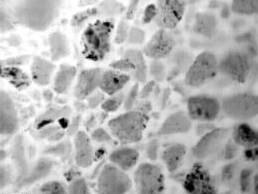
\includegraphics[width=\textwidth]{sample/104_E5R_0}
        \caption{Próbka 104\_E5R\_0}
    \end{subfigure}
    \hspace{0.25cm}
    \vspace{0.5cm}
    \begin{subfigure}{0.3\textwidth}
        \centering
        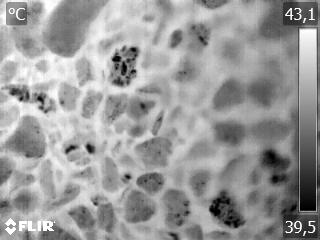
\includegraphics[width=\textwidth]{sample/104_E5R_1}
        \caption{Próbka 104\_E5R\_1}
    \end{subfigure}
    \hspace{0.25cm}
    \begin{subfigure}{0.3\textwidth}
        \centering
        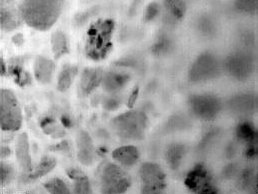
\includegraphics[width=\textwidth]{sample/104_E5R_2}
        \caption{Próbka 104\_E5R\_2}
    \end{subfigure}
    \begin{subfigure}{0.3\textwidth}
        \centering
        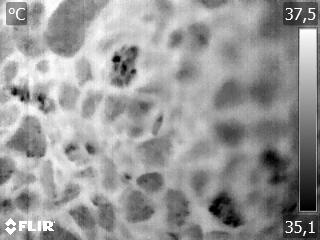
\includegraphics[width=\textwidth]{sample/104_E5R_3}
        \caption{Próbka 104\_E5R\_3}
    \end{subfigure}
    \hspace{0.25cm}
    \vspace{0.5cm}
    \begin{subfigure}{0.3\textwidth}
        \centering
        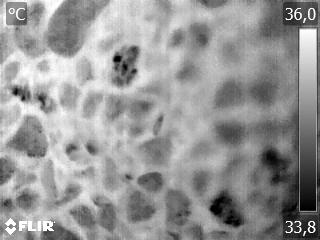
\includegraphics[width=\textwidth]{sample/104_E5R_4}
        \caption{Próbka 104\_E5R\_4}
    \end{subfigure}
    \hspace{0.25cm}
    \begin{subfigure}{0.3\textwidth}
        \centering
        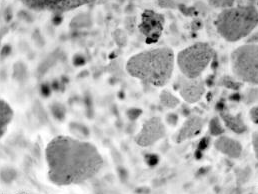
\includegraphics[width=\textwidth]{sample/117_E6R_0}
        \caption{Próbka 117\_E6R\_0}
    \end{subfigure}
    \begin{subfigure}{0.3\textwidth}
        \centering
        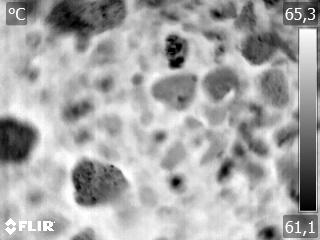
\includegraphics[width=\textwidth]{sample/117_E6R_1}
        \caption{Próbka 117\_E6R\_1}
    \end{subfigure}
    \hspace{0.25cm}
    \vspace{0.5cm}
    \begin{subfigure}{0.3\textwidth}
        \centering
        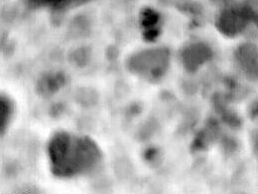
\includegraphics[width=\textwidth]{sample/117_E6R_2}
        \caption{Próbka 117\_E6R\_2}
    \end{subfigure}
    \hspace{0.25cm}
    \begin{subfigure}{0.3\textwidth}
        \centering
        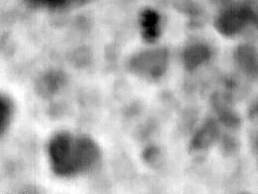
\includegraphics[width=\textwidth]{sample/117_E6R_3}
        \caption{Próbka 117\_E6R\_3}
    \end{subfigure}
    \begin{subfigure}{0.3\textwidth}
        \centering
        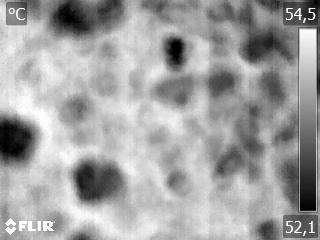
\includegraphics[width=\textwidth]{sample/117_E6R_4}
        \caption{Próbka 117\_E6R\_4}
    \end{subfigure}
    \caption{Porównanie procesu stygnięcia próbek klasy E5R oraz E6R}
    \label{fig:sample_compare}
\end{figure}

\subsection{Wybór cech obrazu użytecznych w~klasyfikacji}
\label{subsec:feature_extraction}
Po przyjrzeniu się rysunkowi \ref{fig:sample_compare}~widoczne jest, że w~próbce
E6R temperatura ziaren zaczęła wyrównywać się szybciej.
Zdjęcia tej próbki wcześniej stają się szare i~tracą kontrast.
Na podstawie analizy nagrań rozpatrzono następujące możliwości ekstrakcji ich
cech charakterystycznych:
\begin{enumerate}[a)]
    \item \label{it:cnn}
          klasyfikacja całych zdjęć z~użyciem zaawansowanych sieci
          konwolucyjnych,
    \item \label{it:fft}
          analiza częstotliwościowa obrazów,
    \item \label{it:glcm}
          użycie macierzy GLCM,
    \item \label{it:edge}
          detekcja krawędzi ziaren i~wyznaczanie reprezentacji liczbowej
          ich kształtów,
    \item \label{it:blob}
          śledzenie zlewania się i~zanikania małych detali na obrazie.
\end{enumerate}
Wszystkie przedstawione opcje mają uzasadnienie i~mogą się dobrze sprawdzić jako
podstawa klasyfikacji.
Metody \ref{it:fft},~\ref{it:glcm}~oraz \ref{it:edge}~były już w~różnym stopniu
badane w~ramach działaności Politechniki Śląskiej \cite{budzan_grains}.
Należy rozpatrzeć, którą technikę wykorzystać do budowy prototypu klasyfikatora.

Metoda bazująca na sieciach konwolucyjnych może wykorzystywać najnowsze
rozwiązania w~dziecinie uczenia maszynowego.
Utrudnieniem w~użyciu tej metody jest bardzo mały rozmiar posiadanego zbioru
danych.
Na zgromadzonych obrazach znajduje się wiele informacji i~szumów, a~złożoność
jednego zdjęcia jest na tę chwilę nieproporcjonalna do wielkości zestawu danych.
Pomysł ten można wypróbować po rozszerzeniu zbioru nagrań.

Technika polegająca na analizie częstotliwościowej obrazów wymaga zastosowania
transformacji Fouriera.
Takie podejście charakteryzuje się złożonością obliczeniową.
Dodatkowo efekt analizy widmowej może być nieoczywisty w~interpretacji.
Wynikiem zastosowania transformacji Fouriera na obrazach są dwuwymiarowe
macierze.
Użycie takich danych wejściowych może wymagać konstrukcji złożonych sieci
neuronowych.
Analizę widmową ziaren przeprowadzono w~pracach naukowców Politechniki Śląskiej,
w~rozpatrywanym przypadku zdecydowano się na poszukiwanie innego rozwiązania.

Macierz GLCM (ang. \textit{Gray-Level Co-Occurrence Matrix}), na której może
bazować opcja \ref{it:glcm},~to tablica zawierająca informacje o~relacjach
wszystkich par pikseli na obrazie.
Pozwala ona na analizę takich wartości jak: kontrast, korelacja, energia oraz
homogeniczność.
Jest to opcja dająca możliwość analizy dużej ilości informacji, z~pewnością
warta rozpatrzenia, jednak dosyć skomplikowana.
Zdecydowano się na wybór mniej złożonej metody.

Na obrazie można także wykrywać kształty ziaren za pomocą filtrów detekcji
krawędzi.
Opcję tę testowano przy pomocy filtra \emph{Canny}.
Uzyskane krawędzie nie pozwalają jednak na łatwą detekcję kształtów.
Tradycyjna segmentacja ziaren jest trudna ze względu na małą rodzielczość oraz
duże upakowanie ziaren.
Operacje morfologiczne domykania kształtów powodowały bardzo duże zmiany
w~obrazie i~zlewały ziarna.
Rozwój takiego podejścia przy analizowanych obrazach wymaga zaawansowanej
i~ostrożnej obróbki zdjęć.

Ostatnia opcja \ref{it:blob}~wynika z~obserwacji detali na obrazach.
Na przedstawionych zdjęciach próbek można zauważyć drobne ciemne punkty, które
są obszarami o~wolniejszej wymianie ciepła z~otoczeniem niż reszta powierzchni
ziaren.
Jest to spowodowane ich niską emisyjnością cieplną.
Na rysunku \ref{fig:blob_detail}~przedstawiono zbliżenie na grupę takich detali,
w~czterech częściach procesu stygnięcia.
\begin{figure}[htb]
    \centering
    \begin{subfigure}{0.3\textwidth}
        \centering
        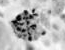
\includegraphics[width=\textwidth]{sample/detail_119_E5R_0}
        \caption{Grupa detali w~próbce 119\_E5R\_0}
    \end{subfigure}
    \hspace{0.25cm}
    \centering
    \begin{subfigure}{0.3\textwidth}
        \centering
        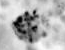
\includegraphics[width=\textwidth]{sample/detail_119_E5R_1}
        \caption{Grupa detali w~próbce 119\_E5R\_1}
    \end{subfigure}
    \hspace{0.24cm}
    \begin{subfigure}{0.3\textwidth}
        \centering
        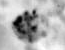
\includegraphics[width=\textwidth]{sample/detail_119_E5R_2}
        \caption{Grupa detali w~próbce 119\_E5R\_2}
    \end{subfigure}
    \caption{Zbliżenie na charakterystyczne grupy detali materiału}
    \label{fig:blob_detail}
\end{figure}

Analizując próbki można zauważyć, że wraz ze stygnięciem, ciemne punkty
w~grupach zlewają się, a~następnie zanikają.
Dodatkowo ich liczba dla poszczególnych klas materiałów jest różna.
Zdecydowano się na wybór metody polegającej na śledzeniu liczby tych punktów
i~ich zaniku.
Taka analiza wiąże się z~przetwarzaniem obrazów i~utworzeniem algorytmów
śledzenia detali.
Opcja ta jest obiecująca, ponieważ nawet podczas wstępnej obserwacji próbek
można dopatrywać się zależności miedzy klasami, a~obecnością omawianych detali.
Można również zaobserwować, że w~czasie stygnięcia na kolejnych zdjęciach
pojawiają się sporadycznie także nowe detale.
Zjawisko ich powstawania jest jednak pomijalne przy zdecydowanej tendencji do
zanika i~rozmywania plam, którą omówiono.
Fakt pojawiania się nowych detali wzięto pod uwagę przy późniejszym procesie
projektowania algorytmów ich śledzenia.

\subsection{Wybór algorytmu detekcji ziaren}
\label{subsec:blob_detect}
Zgodnie z~rozważaniami przedstawionymi w~podsekcji
\ref{subsec:feature_extraction}~%
w~celu klasyfikacji ziaren zdecydowano się na obserwację ilości puntów o~małej
emisyjności
Należy więc wybrać metodę detekcji charakterystycznych elementów.
W~wykrywaniu omawianych detali użyteczne są algorytmy wykrywania plam na
podstawie analizy pochodnych wartości w~obrazie.
Biblioteka Scikit-image udostępnia trzy algorytmy tego typu wykorzystujące:
\begin{enumerate}[a)]
    \item laplasjan funkcji Gaussa,
    \item różnicę funkcji Gaussa,
    \item wyznacznik Hesjanu.
\end{enumerate}
Przedstawione algorytmy pozwalają na wykrycie na obrazie plam o~kształcie
zbliżonym do kolistego oraz oszacowanie ich promieni.
Badane detale, przedstawione na rysunku \ref{fig:blob_detail},~mają kształt
zbliżony do kolistego, więc próba użycia rozpatrywanych algorytmów jest
uzasadniona.
Należy porównać dostępne warianty detekcji i~wybrać algorytm, który działa
najskuteczniej na zgromadzonych próbkach.

Metoda bazująca na laplasjanie funkcji Gaussa jest najdokładniejsza, ale także
najwolniejsza.
Funkcja Gaussa, której wykres ma charakterystyczny kształt krzywej dzwonowej
jest dana wzorem \ref{eq:gaussian},~gdzie:
\begin{description}
    \item[$ \sigma $] to odchylenie standardowe,
    \item[$ \mu $] to wartość średnia.
\end{description}
\begin{equation}
    P(x) = \frac{1}{{\sigma \sqrt {2\pi } }}
    e^{{{ - \left( {x - \mu } \right)^2 }
    \mathord{\left/ {\vphantom {{ - \left( {x - \mu } \right)^2 }
            {2\sigma ^2 }}} \right. \kern-\nulldelimiterspace} {2\sigma ^2 }}}
    \label{eq:gaussian}
\end{equation}
Laplasjan to operator różniczkowy drugiego rzędu.
Omawiany algorytm oblicza wartości funkcji Gaussa dla coraz większego odchylenia
standardowego i~układa je w~sześcianie.
Poszukiwane plamy to lokalne maksima w~tym sześcianie.
Wadą tego rozwiązania jest bardzo wolne wykrywanie dużych plam z~powodu
złożoności obliczeniowej.

Różnica funkcji Gaussa jest metodą podobną do poprzedniej.
Ponownie rozmywa ona obrazy z~narastającymi odchyleniami standardowymi z~użyciem
funkcji Gaussa.
Następnie różnice rozmytych obrazów są układane w~sześcianie, gdzie maksima to
plamy.
Metoda ta jest szybsza i~mniej dokładna od algorytmu bazującego na laplasjanie
funkcji Gaussa, ale podobnie jak ona jest wolna w wykrywaniu dużych elementów.

Ostatnia metoda jest najszybsza, ale najmniej dokładna.
Polega na wyszukiwaniu maksimów w~macierzy Hesjanu, jest to macierz drugich
pochodnych cząstkowych.
Postać takiej macierzy w~n-wymiarowej przestrzeni zmiennych $ x $ przedstawia
wzór \ref{eq:hessian}.~%
Prędkość tej metody nie zależy od wielkości wykrywanych plam, ale małe elementy
mogą nie zostać przez nią wykryte \cite{scikit_reference}.
\begin{equation}
    H = \begin{bmatrix}
        \dfrac{\partial^2 f}{\partial x_1^2} &
        \dfrac{\partial^2 f}{\partial x_1\,\partial x_2} &
        \cdots & \dfrac{\partial^2 f}{\partial x_1\,\partial x_n} \\[2.2ex]
        \dfrac{\partial^2 f}{\partial x_2\,\partial x_1} &
        \dfrac{\partial^2 f}{\partial x_2^2} &
        \cdots & \dfrac{\partial^2 f}{\partial x_2\,\partial x_n} \\[2.2ex]
        \vdots & \vdots & \ddots & \vdots \\[2.2ex]
        \dfrac{\partial^2 f}{\partial x_n\,\partial x_1} &
        \dfrac{\partial^2 f}{\partial x_n\,\partial x_2} &
        \cdots &
        \dfrac{\partial^2 f}{\partial x_n^2}
    \end{bmatrix}
    \label{eq:hessian}
\end{equation}

Porównanie działania wymienionych metod przedstawiono na grafice
\ref{fig:blob_compare}.~%
Zgodnie z~teoretycznym opisem funkcji najlepsza okazała się metoda Laplasjanu
funkcji Gaussa.
Funkcję korzystającą z~wyznacznika Hesjanu należy odrzucić, ponieważ
w~rozważanym przypadku istotne jest wykrywanie małych plam.
Z~tego samego powodu korzystne jest użycie najdokładniejszej funkcji.
Ponieważ program nie powinien wykrywać dużych elementów, nie ma ryzyka zbyt
powolnych obliczeń na obszernych plamach.
\begin{figure}[htb]
    \centering
    \begin{subfigure}[t]{0.3\textwidth}
        \centering
        \input{figures/blob_detection_compare_LoG}
        \caption{Laplasjan funkcji Gaussa}
    \end{subfigure}
    \hfill
    \begin{subfigure}[t]{0.3\textwidth}
        \centering
        \input{figures/blob_detection_compare_DoG}
        \caption{Różnica funkcji Gaussa}
    \end{subfigure}
    \hfill
    \begin{subfigure}[t]{0.3\textwidth}
        \centering
        \input{figures/blob_detection_compare_DoH}
        \caption{Wyznacznik Hesjanu}
    \end{subfigure}
    \caption{Porównanie bibliotecznych algorytmów wykrywania plam na obrazie}
    \label{fig:blob_compare}
\end{figure}

Aby wybrana funkcja laplasjanu funkcji Gaussa wykrywała tylko małe plamy należy
podać jej odpowiednie parametry.
Uczyniono to już na etapie porównania metod detekcji.
Wywołanie omawianej funkcji ma postać przedstawioną na listingu
\ref{lst:find_blobs}.~%
Funkcji podano dwa dodatkowe argumenty, które są istotne dla pożądanego
działania.
Argument \mintinline{python}{max_sigma} ogranicza odchylenie standardowe
obliczanych funkcji Gaussa, przez co wykrywane są tylko małe elementy.
Drugi argument \mintinline{python}{threshold} decyduje o~poziomie, powyżej
którego punkt jest uznany za maksimum w~sześcianie laplasjanów.
Domyślna wartość tego argumentu \mintinline{python}{threshold} okazała się zbyt
duża, zmniejszono ją aby wykrywać bardziej subtelne detale.
Na podstawie opisanego wywołania metody laplasjanu funkcji Gaussa opracowano
funkcję zwracającą położenie i~promienie wykrytych plam.
\begin{listing}[htb]
\begin{minted}{python}
def find_blobs(img):
    '''
    Find blobs in given image and get list of their positions
    and radiuses.
    '''
    # Detect blobs with Difference of Gaussian
    blobs = blob_dog(img, max_sigma=2, threshold=0.1)
    # Get blobs radiuses from each kernel sigma
    blobs[:, 2] = blobs[:, 2] * sqrt(2)
    return blobs
\end{minted}
\caption{Funkcja języka Python wykrywająca detale na obrazie}
\label{lst:find_blobs}
\end{listing}

\subsection{Algorytm śledzenia ziaren w~serii zdjęć}
\label{subsec:blob_tracking}
Użycie funkcji bibliotecznych opisanych w~podsekcji \ref{subsec:blob_detect}~%
pozwala na detekcję detali na pojedynczym zdjęciu.
Aby wykorzystać detekcję plam w~serii pięciu zdjęć, które reprezentują
stygnięcie jednej próbki, należy opracować zestaw funkcji śledzący zmiany na
obrazie.
Na tym etapie prac nie jest jednoznaczne jaki sposób obserwacji i~zliczania
detali będzie najlepszy do późniejszego prototypowania sieci neuronowej
klasyfikującej ziarna rud miedzi.
Dlatego zdecydowano się na napisanie funkcji zliczania plam, tak by umożliwić
trzy warianty pracy algorytmu:
\begin{enumerate}[a)]
    \item \label{it:all_blob}
          zliczanie wszystkich detali na każdym etapie stygnięcia,
    \item \label{it:remaining_blob}
          zliczanie detali śledzonych od początku stygnięcia,
    \item \label{it:ratio_blob}
          zliczanie stosunku śledzonych detali do ich ilości na początku
          stygięcia.
\end{enumerate}
Przez śledzenie detali rozumiane jest zliczanie jedynie tych plam, które były
wykryte na początku stygnięcia.
Oznacza to, że metody \ref{it:remaining_blob}~oraz \ref{it:ratio_blob}~ignorują
detale pojawiające się w~późniejszych etapach studzenia ziaren.

W~celu realizacji planu śledzenia detali utworzono funkcję języka Python.
Jej kod przedstawiono na listingu \ref{lst:find_blob_series}.~%
Aby umożliwić wariantowość algorytmu funkcja posiada opcjonalny parametr, który
pozwala aktywować śledzenie wyłącznie tych ziaren, które były obecne od początku
stygnięcia.
Omawiany kod wykorzystuje funkcję wykrywania detali na zdjęciu przedstawioną na
listingu \ref{lst:find_blobs}.~%
\begin{listing}[htb]
\begin{minted}{python}
def find_blob_series(imgs, only_remaining=True):
    '''
    Return list of list of blobs found in each of given images.
    '''
    stages = []
    remaining = None
    for img in imgs:
        new_blobs = find_blobs(img)
        if remaining is not None and only_remaining:
            remaining = find_remaining_blobs(new_blobs, remaining)
        else:
            remaining = new_blobs
        stages.append(remaining)
    return stages
\end{minted}
\caption{Funkcja języka Python śledząca detale w~serii zdjęć}
\label{lst:find_blob_series}
\end{listing}
Wybór opcji detekcji ziaren obecnych jedynie od początku stygnięcia, powoduje
wywołanie funkcji porównania wykrytych detali, z~punktami na poprzednim zdjęciu.
Po analizie każdego zdjęcia nowy zestaw ziaren staje się zbiorem poprzednim
w~kolejnej iteracji.
Dzieje się tak, by uwzględnić fakt że podczas zlewania się ziaren środki
ciężkości i~promienie detali ulegają zmianie.
Dlatego kolejne grupy plam nie są zawsze porównywane z~grupą z~początku serii,
a~z~zestawem z poprzedniego analizowanego zdjęcia.

Na listingu \ref{lst:find_remaining_blobs}~przedstawiono funkcję testującą,
które z~detali znajdują się na kolejnych etapach stygnięcia.
\begin{listing}[htb]
\begin{minted}{python}
def find_remaining_blobs(new_blobs, old_blobs):
    '''
    Return list of blobs present in both lists, where blob
    is considered same if is in proximity of 2 times it's radius.
    '''
    remaining = []
    for new_blob in new_blobs:
        yn, xn, _ = new_blob
        for old_blob in old_blobs:
            yo, xo, ro = old_blob
            if inside_circle(xn, yn, xo, yo, 2 * ro):
                remaining.append(new_blob)
    return unique(remaining)\end{minted}
\caption{Funkcja języka Python wykrywające te same detale w~kolejnych
    obrazach}
\label{lst:find_remaining_blobs}
\end{listing}
Przyjmuje ona listy plam wykrytych w~dwóch kolejnych etapach iteracji.
Potem następuje porównanie każdego ziarna z~nowej i~starej próbki.
Jeżeli nowy punkt znajduje się w~odległości do dwóch promieni od środka starej
plamy, to zostaje on uznany za powtarzający się.
Powtarzające się punkty są dołączane do zwracanej listy.
Aby zrealizować ten zamysł zaimplementowano funkcję przedstawioną na listingu
\ref{lst:inside_circle}.~%
\begin{listing}[htb]
\begin{minted}{python}
def inside_circle(x, y, a, b, r):
    '''
    Return True if point (x, y) lies inside circle
    with center of (a, b) and radius r.
    '''
    return (x - a) * (x - a) + (y - b) * (y - b) < r * r
\end{minted}
\caption{Funkcja języka Python sprawdzająca czy dany punkt leży wewnątrz
    podanego okręgu}
\label{lst:inside_circle}
\end{listing}
Kod tej funkcji wynika wprost z~równania matematycznego okręgu.
Ponieważ wiele punktów może znajdować się blisko siebie istnieje ryzyko, że
zostaną one zliczone wiele razy.
Z~tego powodu przed zwróceniem listy należy usunąć z~niej duplikaty.
W~tym celu utworzono funkcje pomocniczą widoczną na listingu \ref{lst:unique}.~%
\begin{listing}[htb]
\begin{minted}{python}
def unique(multilist):
    '''Get list without repeating values.'''
    return list(set(tuple(i) for i in multilist))    \end{minted}
\caption{Funkcja języka Python usuwająca duplikaty z~listy}
\label{lst:unique}
\end{listing}
Najprostszym sposobem eliminacji powtarzających się wartości w~języku Python
jest konwersja listy na zbiór, który jest agregatem unikalnych nieuszeregowanych
wartości.
Aby zwrócić z~funkcji listę należy z~powrotem skonwertować zbiór na typ listowy.
W~naszym przypadku argument funkcji jest listą, której elementy są listami
zawierającymi współrzędne oraz promień każdej plamy.
Lista list nie podlega konwersji do zbioru, ponieważ typ jej elementów nie
posiada funkcji hashowania.
Dlatego każdy punkt na liście zamieniono uprzednio w~typ krotki.
W~ten sposób wszystkie konieczne przekształcenia są możliwe.
Aby zrealizować pomysł liczenia stosunku plam pozostałych w~kolejnych etapach
stygnięcia zaimplementowano funkcję przedstawioną na listingu \ref{lst:ratio}.
\begin{listing}[htb]
\begin{minted}{python}
def ratio_of_remaining_blobs_in_stages(stages):
    '''
    In each stage calculate ratio of remaining blobs
    to their initial number.
    '''
    num_of_blobs = [len(stage) for stage in stages]
    return [remaining / num_of_blobs[0] for remaining in num_of_blobs]
\end{minted}
\caption{Funkcja języka Python obliczająca jaka część ziaren z~początku
    stygnięcia pozostała w~jego kolejnych etapach}
\label{lst:ratio}
\end{listing}

Przyglądając się zaimplementowanym funkcjom można docenić wybór języka
Python do realizacji projektu.
Elastyczność języka Python, w~szczególności jego list oraz wygoda dynamicznego
typowania pozwoliły na szybkie i~eleganckie zaimplementowanie potrzebnych
funkcji.
Wykorzystano bardzo zwięzły i~ekspresyjny element języka nazywany
\emph{wyrażeniami listowymi}.
Pozwala on na efektywne stosowanie jedno-linijkowych pętli do przeglądania
i modyfikowania obiektów iterowalnych.
Użyteczność tego mechanizmu można zaobserwować na przedstawionych listingach.

Przedstawiony zestaw funkcji daje możliwość ekstrakcji liczby plam, w~serii
zdjęć, na trzy sposoby.
Efekty działania utworzonego kodu przetestowano na obrazach pomiarowych.
Działanie sposobów zliczania ziaren \ref{it:all_blob}~oraz
\ref{it:remaining_blob}~przedstawiono na rysunku \ref{fig:blob_count}.~%
Zaznaczono na nim wykryte detale oraz wyróżniono wśród nich, te które są
śledzone od początku stygnięcia.
\begin{figure}[htbp]
    \centering
    \hfill
    \begin{subfigure}[t]{0.45\textwidth}
        \centering
        \caption*{\scriptsize
            Minuta: 0, \\
            Liczba: wszystkich detali: 56, śledzonych detali: 56}
        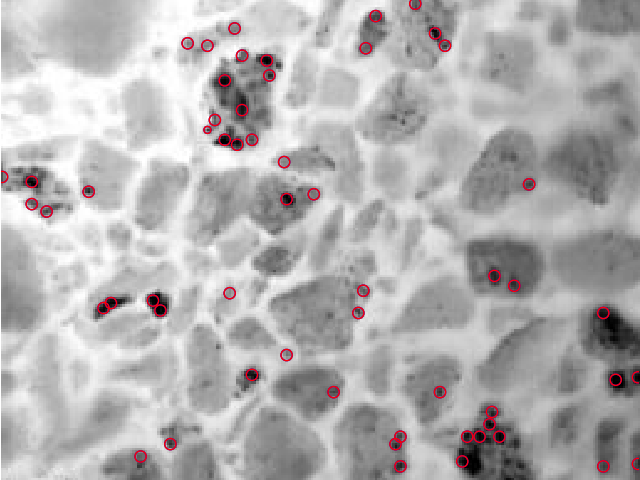
\includegraphics[width=0.8\textwidth]{blob_tracker_min_0}
        \caption{Obraz z~próbki 104\_E5R\_0}
    \end{subfigure}
    \hfill
    \begin{subfigure}[t]{0.45\textwidth}
        \centering
        \caption*{\scriptsize
            Minuta: 0, \\
            Liczba: wszystkich detali: 36, śledzonych detali: 29}
        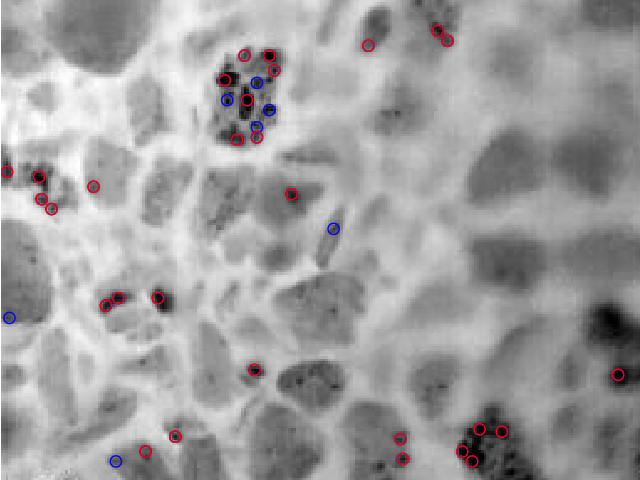
\includegraphics[width=0.8\textwidth]{blob_tracker_min_1}
        \caption{Obraz z~próbki 104\_E5R\_1}
    \end{subfigure}
    \hfill
    \vfill
    \hfill
    \begin{subfigure}[t]{0.45\textwidth}
        \centering
        \caption*{\scriptsize
            Minuta: 0, \\
            Liczba: wszystkich detali: 22, śledzonych detali: 16}
        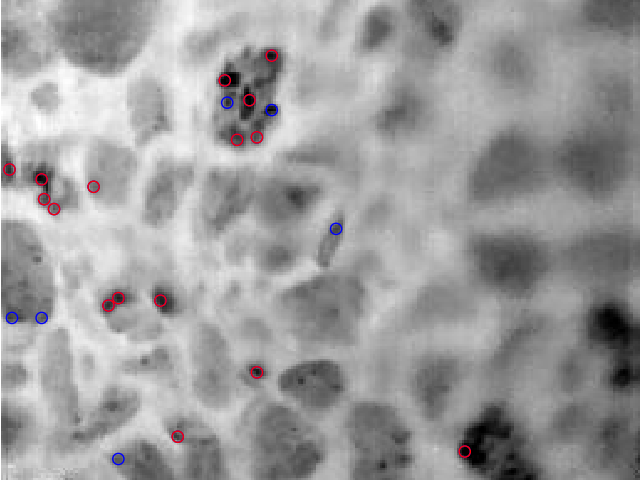
\includegraphics[width=0.8\textwidth]{blob_tracker_min_2}
        \caption{Obraz z~próbki 104\_E5R\_2}
    \end{subfigure}
    \hfill
    \begin{subfigure}[t]{0.45\textwidth}
        \centering
        \caption*{\scriptsize
            Minuta: 0, \\
            Liczba: wszystkich detali: 19, śledzonych detali: 13}
        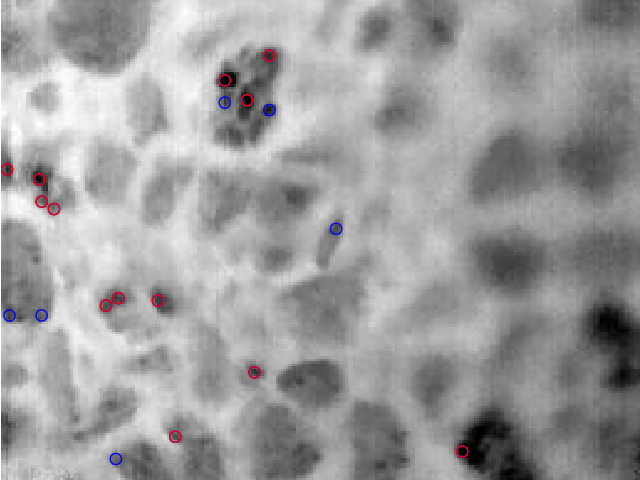
\includegraphics[width=0.8\textwidth]{blob_tracker_min_3}
        \caption{Obraz z~próbki 104\_E5R\_3}
    \end{subfigure}
    \hfill
    \vfill
    \begin{subfigure}[t]{0.45\textwidth}
        \centering
        \caption*{\scriptsize
            Minuta: 0, \\
            Liczba: wszystkich detali: 15, śledzonych detali: 11}
        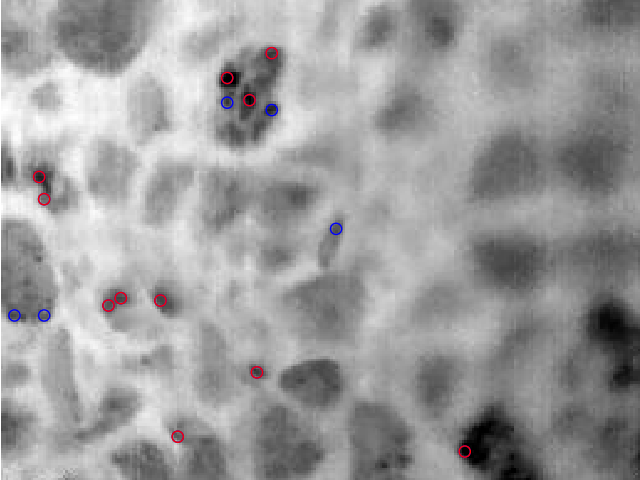
\includegraphics[width=0.8\textwidth]{blob_tracker_min_4}
        \caption{Obraz z~próbki 104\_E5R\_4}
    \end{subfigure}
    \begin{description} \footnotesize
        \centering
        \item[Kolor czerwony] detale śledzone od początku stygnięcia
        \item[Kolor niebieski] nowe wykryte detale
    \end{description}
    \caption{Zliczanie śledzonych detali w~próbce dwoma sposobami}
    \label{fig:blob_count}
\end{figure}

Metodę śledzenia plam i~ich zanikania przedstawiono na rysunku
\ref{fig:blob_remain}.~%
Pokazuje on położenie plam wykrytych w~kolejnych etapach stygnięcia.
Wykryte punkty zaznaczono na obrazie z~początku tego procesu.
Zmieniające się kolory obrazują detale wykryte w~kolejnych chwilach.
Pozawala to zaobserwować przemieszczanie się środków ciężkości i~promieni plam
podczas stygnięcia i zlewania się.
\begin{figure}[htb]
    \centering
    \caption*{\scriptsize Detekcja metodą laplasjanu funkcji Gaussa}
    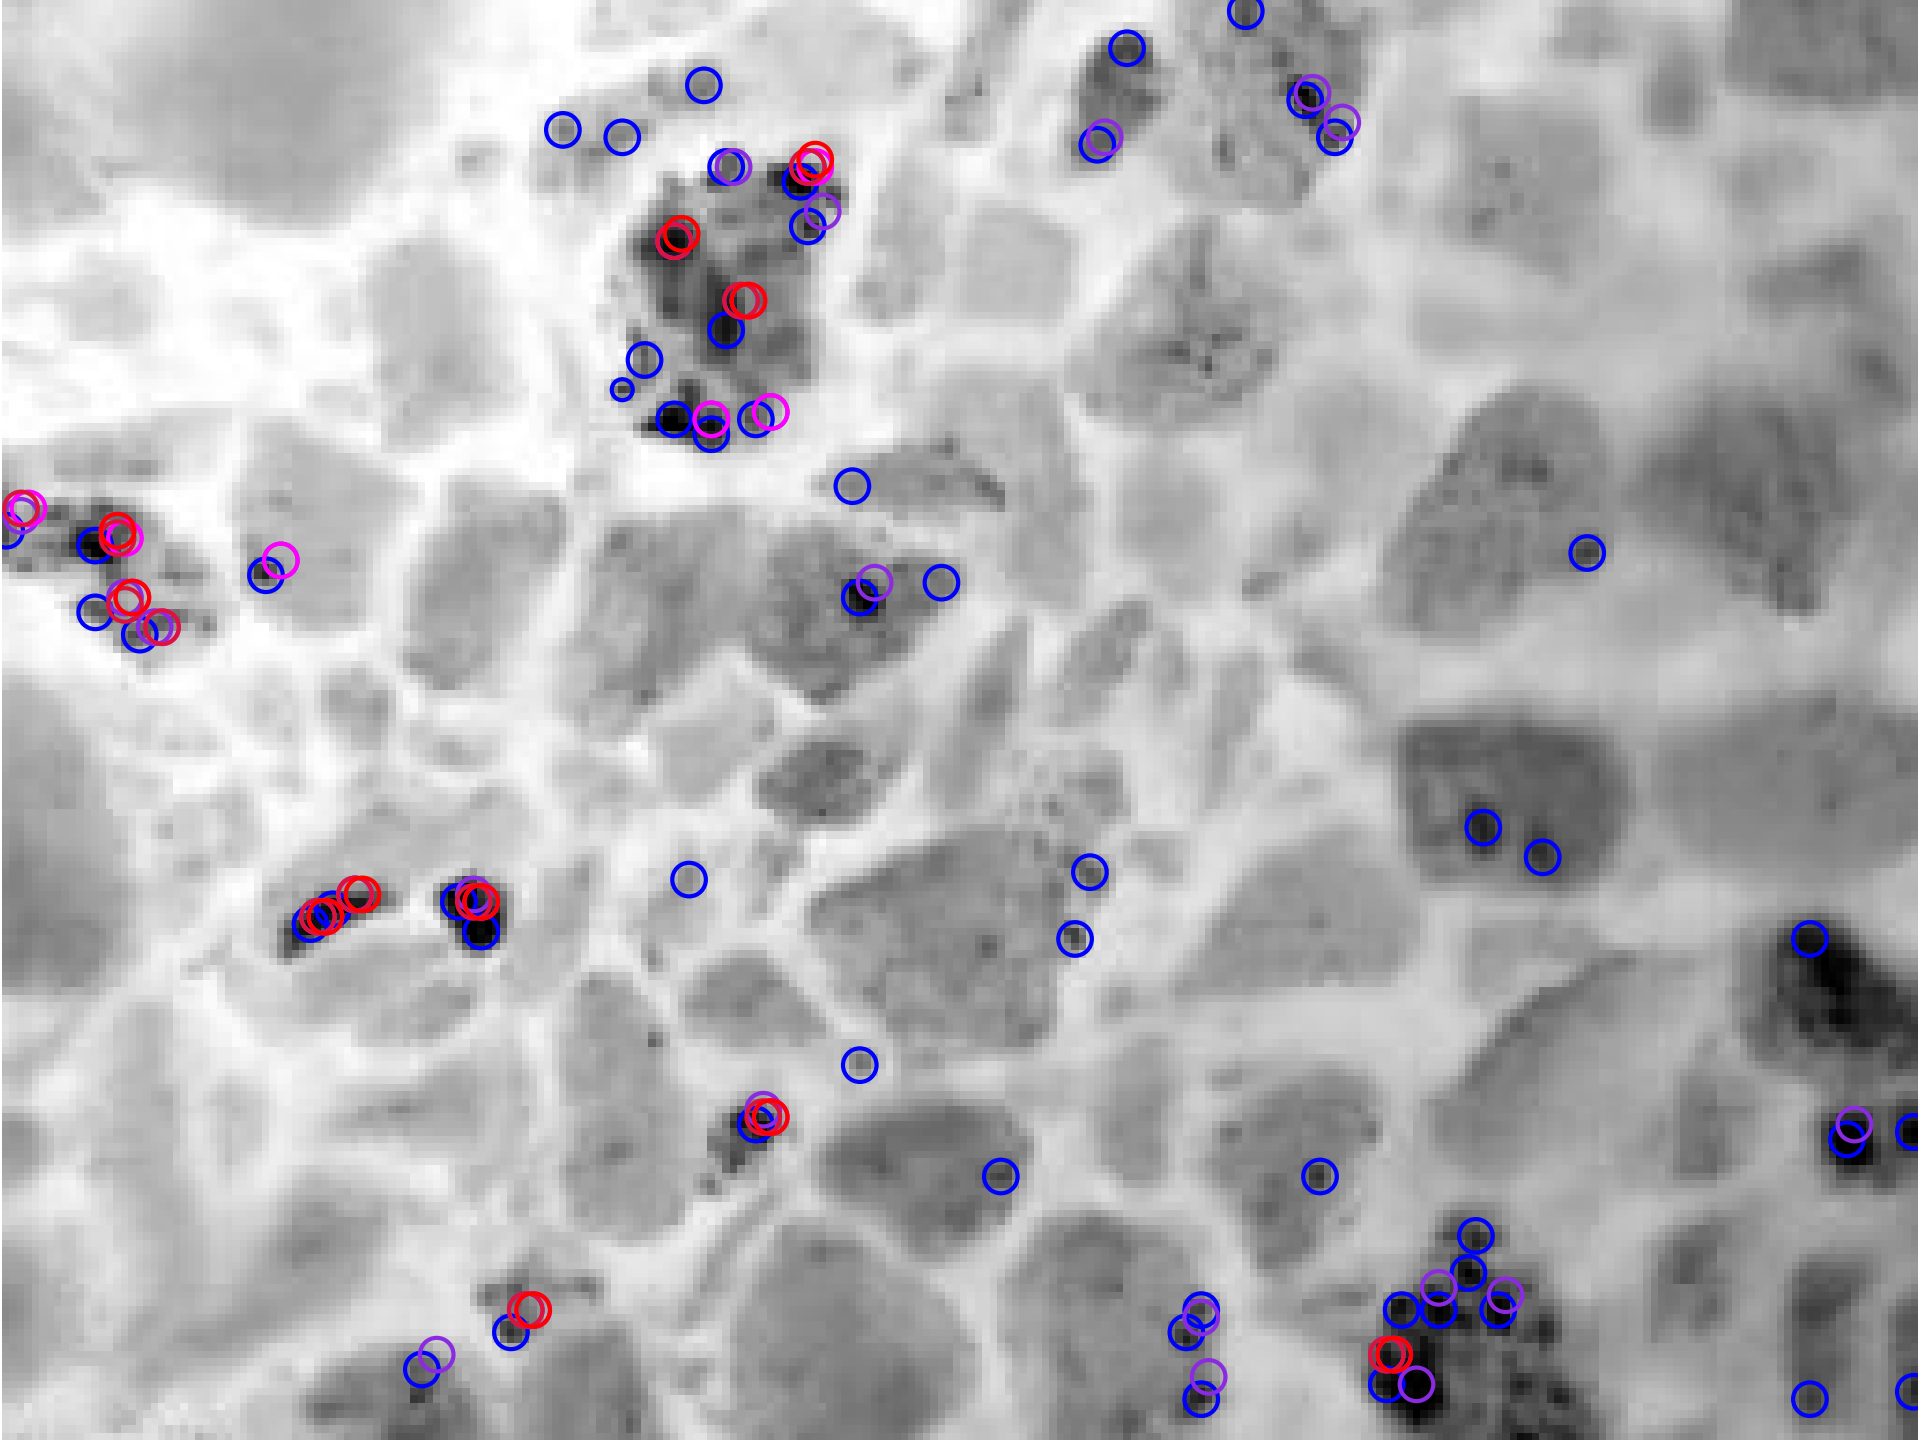
\includegraphics[width=0.5\textwidth]{blob_tracker}
    \vspace{0.3cm}
    \caption*{\scriptsize
        Kolorem niebieskim zaznaczono detale wykryte na początku stygnięcia.
        Wraz z~upływem czasu kolor oznaczenia detali przechodzi w~czerwień}
    \caption{Wykryte detale, śledzone od początku stygnięcia, zaznaczone na
        pierwszym obrazie w~serii pomiarowej}
    \label{fig:blob_remain}
\end{figure}
Działanie metody \ref{it:ratio_blob},~zliczającej stosunek śledzonych detali
do ich pierwotnej liczby zobrazowano w~tabeli \ref{tab:blob_ratio}.~%
Działanie zliczania przedstawiono dla każdej rozpatrywanej klasy ziaren.
\begin{table}[htb]
    \centering
    \begin{tabular}{c|c|c|c|c|c}
        \toprule
        Próbka    & Minuta 0 & Minuta 1 & Minuta 2 & Minuta 3 & Minuta 4 \\ \midrule
        104\_E5R  & 1.0      & 0.52     & 0.29     & 0.23     & 0.20     \\
        107\_E6R  & 1.0      & 0.20     & 0.12     & 0.02     & 0.02     \\
        106\_E11R & 1.0      & 0.12     & 0.02     & 0.00     & 0.00     \\
        111\_E16R & 1.0      & 0.05     & 0.01     & 0.01     & 0.01     \\
        \bottomrule
    \end{tabular}
    \caption{Stosunek liczby detali śledzonych w~kolejnych etapach stygnięcia do
        ich liczby na początku pomiaru}
    \label{tab:blob_ratio}
\end{table}

\subsection{Wizualizacja zebranych cech i~ocena ich użyteczności}
\label{subsec:data_vis}
W~podsekcji \ref{subsec:blob_tracking}~przedstawiono opracowane algorytmy
śledzenia ilości detali w~rozpatrywanych obrazach stygnięcia ziaren rud miedzi.
Opracowane metody mają sens przy klasyfikacji, jeśli pozyskane cechy są
charakterystyczne dla rozpatrywanych klas.
Aby oszacować użyteczność pozyskanych cech należy przeprowadzić ich
wizualizację.
W~tym celu stworzono wykresy ilości wykrytych plam dla poszczególnych metod ich
zliczania.

Rysunek \ref{fig:blob_chart_all}~przedstawia wykres procesu zanikania plam dla
wariantu z~wykrywaniem wszystkich detali na każdym etapie stygnięcia.
\begin{figure}[htb]
    \centering
    \input{figures/blob_analysis_all}
    \caption{Liczba wykrytych detali na~każdym etapie stygnięcia, w~wariancie
        zliczającym wszystkie plamy}
    \label{fig:blob_chart_all}
\end{figure}
Wykreślone krzywe dla różnych klas materiałów przecinają się, na wykresach nie
widać uporządkowania, ani wyraźnych zależności.
Liczba charakterystycznych detali może być cechą ziaren rud miedzi, ze względu
na ich różną budowę, jednak w~analizowanym przypadku nie jest to cecha dająca
nadzieję na dobre wyniki klasyfikacji.
Powodem takiej sytuacji jest duża losowość tego typu danych.
Niezależnie od własności materiału, jego ułożenie podczas pomiaru jest
przypadkowe, co ma wpływ na bezwzględną liczbę zliczonych detali.
Na liczbę widocznych plam wpływa również sposób ustawienia ostrości kamery.
Po przyjrzeniu się wykresom można jednak domniemywać, że pewną cechą
charakterystyczną jest nachylenie krzywych.
Wskazuje to, że bardziej widoczne mogą być względne cechy czasowe, a~nie
bezwzględna liczba zliczonych detali.

Efekty drugiego sposób zliczania punktów przedstawiono na rysunku
\ref{fig:blob_chart_rem}.~%
\begin{figure}[htb]
    \centering
    \input{figures/blob_analysis_remaining}
    \caption{Liczba detali wykrytych na zdjęciach, w~wariancie zliczającym
        plamy śledzone od początku procesu stygnięcia}
    \label{fig:blob_chart_rem}
\end{figure}
W~tym przypadku zliczano jedynie detale obecne na obrazie od początku
stygnięcia.
Ten wariant śledzenia ilości plam daje dużo lepsze perspektywy na klasyfikację
ziaren.
Dla różnych typów próbek widoczne są charakterystyczne przebiegi krzywych.
Obserwacja dotycząca nachylenia krzywych staje się bardziej uzasadniona,
pochodne poszczególnych klas wydają się zbliżone.
Wyeliminowanie pojawiających się detali pomogło w~obserwacji procesu stygnięcia
i~zmniejszyło czynniki losowe.
Na podstawie analizy nagrań można domniemywać, że nowe ziarna pojawiały się
w~wyniku zaobserwowanych delikatnych ruchów materiału.
Te mogły wynikać z~drgań stanowiska pomiarowego, istotnym czynnikiem może być
także mała głębia ostrości obiektywu.
W~późniejszych etapach stygnięcia na obrazach pojawia się także coraz więcej
szumów, które mogą zostać wykryte przez algorytm.
Śledzenie detali, które znajdują się na obrazie od początku eliminuje ten
problem.

Wyniki ostatniej metody, polegającej na ustaleniu stosunku śledzonych detali
do ich pierwotnej liczby, został przedstawiona na rysunku
\ref{fig:blob_chart_ratio}.~%
\begin{figure}[htb]
    \centering
    \input{figures/blob_analysis_ratio}
    \caption{Stosunek śledzonych detali do ich liczby na początku procesu
        stygnięcia}
    \label{fig:blob_chart_ratio}
\end{figure}
Widoczne jest odseparowanie różnych klas rud miedzi, różne typy próbek
charakteryzują się odmiennymi postępami rozmycia detali w~czasie.
Śledzenie ilości detali w~stosunku względnym dało najlepsze rezultaty.
Nastąpiła także pewna normalizacja danych, która była trudna do realizacji przy
bezwzględnym zliczaniu wszystkich plam na obrazie.
Należy także zauważyć, że przedstawione krzywe przedstawione na rysunkach
\ref{fig:blob_chart_rem}~oraz \ref{fig:blob_chart_ratio}~mają kształt zbliżony
do krzywych eksponencjalnych.
Jest to obserwacja wskazująca, że pozyskane cechy dobrze oddają naturę procesu
stygnięcia.
Proces opadania temperatury ciał opisuje \emph{prawo stygnięcia Newtona}, które
ma postać równania różniczkowego, przedstawionego we wzorze
\ref{eq:newton_law_diff}~\cite{lienhard_heat}, gdzie:
\begin{description}
    \item $ T \left( t \right) $ to funkcja temperatury ciała w~czasie,
    \item $ T_R $ to temperatura otocznia,
    \item $ k $ to współczynnik liczbowy, charakterystyczny dla danego ciała.
\end{description}

\begin{equation}
    \frac{dT \left( t \right)}{dt}=-k\left( T \left( t \right) -T_{R} \right)
    \label{eq:newton_law_diff}
\end{equation}
Rozwiązanie równania przedstawia wzór \ref{eq:newton_law},~jak widać ma ono
charakter eksponencjalny, do którego zbliżone są wykresy na rysunkach
\ref{fig:blob_chart_rem}~oraz \ref{fig:blob_chart_ratio}.
\begin{equation}
    T(t) - T_{R} = \Delta T (t) = \Delta T (0) \ e^ {-k t}
    \label{eq:newton_law}
\end{equation}

Analiza pozyskanych cech wskazuje, że istnieje możliwość ich wykorzystania
w~klasyfikacji rud miedzi.
Dalsza ocena wyników pracy będzie zależała od jakości działania sieci neuronowej
stworzonej do rozpoznawania przygotowanych danych.


\chapter{Prototypowanie sieci neuronowej klasyfikującej ziarna miedzi}
\section{Konstrukcja prototypu sieci neuronowej}
Po zakończeniu procesu eksploracji danych można przystąpić do
konstrukcji sieci neuronowej odpowiedzialnej za rozpoznawanie ziaren rud
miedzi.
Przedstawiony problem wymaga klasyfikacji wieloklasowej wielowymiarowych
danych.
Problemy tego typu można rozwiązywać zarówno za pomocą klasycznych algorytmów
uczenia maszynowego jak i~uczenia głębokiego.
Zdecydowano się na wybór sieci neuronowych do klasyfikacji ziaren.
Jest to rozwiązanie najbardziej nowoczesne i~elastyczne.
Zgodnie z~opisem narzędzi programistycznych w~podsekcji
\ref{subsec:software_network}, proces budowania sieci oparto na interfejsie
Keras, z~zapleczem TensorFlow.

\subsection{Dobór struktury sieci} \label{subsec:nnbuild}
Kluczowym czynnikiem decydującym o~architekturze sieci jest posiadany
zbiór danych.
Wejściowy zestaw cech klas jest pięciowymiarowy, do klasyfikacji takich
danych wystarczająca powinna być standardowa sieć neuronowa.
Nie ma potrzeby używania bardziej złożonych sieci rekurencyjnych, czy
konwolucyjnych.

Projektowanie sieci neuronowych wymaga podjęcia szeregu wyborów, wśród nich
można wyróżnić następujące decyzje dotyczące:
\begin{itemize}
	\item ilości warstw sieci,
	\item typu warstw w sieci,
	\item ilości neuronów w~poszczególnych warstwach sieci,
	\item rodzajów funkcji aktywacji w~neuronach poszczególnych warstw sieci.
\end{itemize}
Definiując model należy rozpatrzeć przedstawione cechy budowanej sieci.
Nie istnieje jednoznaczny sposób bezpośredniego określenia najlepszego
klasyfikatora dla danego problemu.
Przy projektowaniu sieci należy kierować się przesłankami teoretycznymi,
doświadczeniem oraz testując i~porównując różne rozwiązania.
Przedstawiona konstrukcja oraz uzasadnienie jej wyboru bazuje na wynikach
walidacji, której mechanizm przedstawiono w~sekcji \ref{sec:validation}.
Szczegółowe dane, dotyczące porównań różnych konstrukcji i~parametrów
sieci przedstawiono w~dodatku \ref{ch:nn_comparison_table}.

Konstrukcję klasyfikatora rozpoczęto od wyboru ilości warstw.
W~standardowej konstrukcji każda sieć posiada warstwę wejściową oraz
wyjściową, których parametry są związane odpowiednio z~wektorem cech
oraz reprezentacją klas na wyjściu sieci.
Aby zwiększać efektywność sieci pomiędzy warstwą wejściową oraz wyjściową
umieszcza się zestaw warstw nazywanych \emph{ukrytymi}.
Zazwyczaj posiadają one najwięcej neuronów spośród warstw w~sieci.
Matematycznie dowiedziono, że jedna warstwa ukryta \footnote{Przy
pewnych obostrzeniach co do doboru funkcji aktywacji.} wystarcza do
aproksymacji dowolnej funkcji nieliniowej \cite{cybenko_approximations}.
Nie oznacza to jednak, że w~praktyce tak mała sieć wystarczy, aby rozwiązać
dowolny problem uczenia maszynowego.
Dodanie większej ilości warstw ukrytych jest jednym z~najlepszych sposobów na
poprawę działania sieci w~realnych warunkach \cite[str. 273]{geron_ml}.
Biorąc pod uwagę złożoność rozpatrywanego problemu zdecydowano się na
strukturę czterowarstwową (warstwa wejściowa, wyjściowa i~dwie warstwy
ukryte).
Jest to rozmiar często spotykany w~sieciach tego typu, późniejsze testy
pokazały, że wybrana liczba warstw daje dobre rezultaty.
Sprawdzono, że zastosowanie jednej warstwy ukrytej powodowało pogorszenie
działania sieci.

Kolejnym krokiem projektowania sieci jest decyzja o~ilości neuronów
w~poszczególnych warstwach.
W przypadku pierwszej i~ostatniej warstwy jest to wartość prosta do
określenia.
Zaleca się, aby wejście sieci miało liczbę neuronów równą liczbie elementów
wektora cech, który w~rozpatrywanym przypadku ma długość równą pięć 
\cite[str. 272]{geron_ml}.
Ostatnia warstwa powinna mieć tyle neuronów ile wynosi liczba rozpoznawanych
klas, tak by każde wyjście sieci oznaczało prawdopodobieństwo przynależności
próbki do odpowiedniej klasy.
W~analizowanym zbiorze ziaren znajdują się cztery typy rud miedzi i~tyle
neuronów powinno znajdować się w~warstwie wyjściowej sieci.
W~warstwach ukrytych umieszczono większą liczbę neuronów, eksperymentalnie
stwierdzono, że sieć osiąga dobre wyniki dla 256 neuronów w~pierwszej
warstwie ukrytej i~128 w~drugiej.
Zmniejszenie liczby neuronów w~kolejnej warstwie ukrytej jest
często spotykanym zabiegiem.
Obecnie w~skomplikowanych sieciach coraz częściej stosuje się tę samą
liczbę neuronów w~warstwach ukrytych w~celu łatwiejszej parametryzacji
modelu \cite[str. 272]{geron_ml} .
Ponieważ w~rozpatrywanym przypadku liczba warstw jest niewielka, zrezygnowano
z~tej praktyki i~zdecydowano się na podejście polegające na zmniejszeniu
liczby neuronów w~drugiej warstwie ukrytej.


Następnie rozpatrzono dostępne funkcje aktywacji poszczególnych warstw.
Dla warstwy wyjściowej należy wybrać funkcję o~wartościach od zera do jeden.
Jest to uzasadnione faktem, że wyjścia powinny reprezentować
prawdopodobieństwo zaliczenia próbki do danej klasy.
Przy klasyfikacji zazwyczaj stosuje się funkcję softmax, jej wykres
przedstawiono na rysunku \ref{fig:softmax}.
\begin{figure}[htb]
\centering
\begin{tikzpicture}[trim axis left]
    \begin{axis}[title={$ Softmax(z) $}, width=8cm, height=6cm,
                 ylabel=$ \sigma(z) $, xlabel=$ z $, xmin=-5, xmax=5]
       \addplot[blue, domain=-5:5, samples=51] 
       {exp(x) / sumexp(x, -4, 0)};
    \end{axis}
\end{tikzpicture}
\caption{Funkcja aktywacji softmax}
\label{fig:softmax}
\end{figure}
W~przypadku pozostałych warstw wybór funkcji aktywacji jest mniej oczywisty.
Rozpatrzono trzy rodziny funkcji:
\begin{itemize}
	\item funkcję sigmoid,
	\item funkcje z~grupy jednostek liniowych (ang. \emph{linear unit}):
		\begin{itemize}	
        	\item ReLU (ang. \emph{Rectified Linear Unit}),
        	\item ELU (ang. \emph{Exponential Linear Unit}),
        \end{itemize}
	\item funkcję tangens hiperboliczny.
\end{itemize}
Rozpatrywane funkcje aktywacji przedstawiono na rysunku \ref{fig:activation}.
\begin{figure}[htb]
\centering
\begin{subfigure}[t]{0.3\textwidth}
\centering
\begin{tikzpicture}[trim axis left]
    \begin{axis}[title={$ Sigmoid(z) $}, width=5cm, height=4cm,
                 ylabel=$ \sigma(z) $, xlabel=$ z $, xmin=-5, xmax=5]
       \addplot[blue, domain=-5:5, samples=51] 
       {1 / (1 + e^(-x)};
    \end{axis}
\end{tikzpicture}
\caption{Funkcja aktywacji tangens hiperboliczny}
\end{subfigure}
\hspace{0.25cm}
\begin{subfigure}[t]{0.3\textwidth}
\centering
\begin{tikzpicture}[trim axis left]
    \begin{axis}[title={$ LU(z) $}, width=5cm, height=4cm,
                 ylabel=$ \sigma(z) $, xlabel=$ z $, xmin=-3, xmax=3,
                 legend style={at={(0.02, 0.98)}, anchor=north west}]
       \addplot[red, domain=-3:3, samples=31] 
       {max(0, x)};
       \addplot[blue, domain=-3:3, samples=31] 
       {x < 0 ? 0.1*(e^x - 1) : x};
    \legend{ReLU, ELU}
    \end{axis}
\end{tikzpicture}
\caption{Rodzina funkcji aktywacji jednostek liniowych}
\end{subfigure}
\hspace{0.25cm}
\begin{subfigure}[t]{0.3\textwidth}
\centering
\begin{tikzpicture}[trim axis left]
    \begin{axis}[title={$ Tanh(z) $}, width=5cm, height=4cm,
                 ylabel=$ \sigma(z) $, xlabel=$ z $, xmin=-5, xmax=5]
       \addplot[blue, domain=-5:5, samples=51] 
       {tanh(x)};
    \end{axis}
\end{tikzpicture}
\caption{Funkcja aktywacji tangens hiperboliczny}
\end{subfigure}
\caption{Funkcje aktywacji rozpatrywane do użycia w~warstwach
         ukrytych}
\label{fig:activation}
\end{figure}
Funkcja sigmoid jest często stosowaną, klasyczną funkcją aktywacji.
Jej wadą jest jednak zanikanie wartości pochodnej.
Obecnie częściej stosowane są funkcję z~rodziny jednostek liniowych,
szczególnie z wyciekiem, czyli małymi wartościami dla ujemnych argumentów.
Przetestowano również funkcję tangens hiperboliczny, która ma kształt
podobny do funkcji sigmoid.
Mimo, że obecnie funkcje jednostek liniowych są najbardziej popularne
w~rozpatrywanym przypadku sieć osiągała najlepsze wyniki dla funkcji tangens.

Opisany model sieci neuronowej należy zdefiniować za pomocą interfejsu
Keras.
Do inicjalizacji sieci o~standardowej liniowej strukturze służy funkcja
\mintinline{python}{Sequential()}, która może przyjąć listę warstw w~sieci.
Funkcja \mintinline{python}{Dense()} tworzy warstwę łącząca każdy neuron
z~każdym wyjściem poprzedniej warstwy.
Jej parametry definiują liczbę neuronów w~warstwie oraz ich funkcję aktywacji.
Funkcję języka Python implementują opisywaną sieć, za pomocą przedstawionych
elementów biblioteki Keras, przedstawiono na listingu \ref{lst:model}.
\begin{listing}[htb]
\begin{minted}{python}
def default_grain_classifier_model():
    '''
    Get default uncompiled model for grain classifcation,
    based on 5 step cooling process using number of blobs.
    '''
    model = keras.Sequential([
        keras.layers.Dense(5, activation='tanh'),
        keras.layers.Dense(256, activation='tanh'),
        keras.layers.Dense(128, activation='tanh'),
        keras.layers.Dense(4, activation='softmax')
    ])
    return model
\end{minted}
\caption{Funkcja języka Python definiująca model sieci neuronowej}
\label{lst:model}
\end{listing}

\subsection{Trening sieci neuronowej}
\label{subsec:train}
Kolejnym krokiem w~budowie klasyfikatora ziaren jest trening sieci neuronowej.
Jest to proces. w~którym wagi neuronów są dopasowywane do zbioru uczącego.
Rozpatrywany problem jest typu uczenia nadzorowanego.
Przygotowane dane mają znane etykiety klas, to znaczy są odgórnie przypisane
do danego typu.
Narzucone etykiety nazywane są \emph{wiedzą ekspercką}, ich prawdziwość jest
pewna.
Etykiety przypisane przez klasyfikator będą oceniane przez porównanie
z~etykietami eksperckimi.
Trening polega na zbliżaniu wyników działania sieci do etykiet zbioru
uczącego.

Przed rozpoczęciem uczenia sieci należy podzielić dostępne dane na zbiór
treningowy oraz~testowy.
W~skład zbioru testowego nie powinny wchodzić dane uczące.
Ocena zdolności sieci do generalizacji problemu może bazować tylko
na danych, które nie brały udziału w~jej treningu.
Aby ułatwić podział Biblioteka Scikit-learn udostępnia funkcję
\mintinline{python}{train_test_split()}, która zwraca
podane zbiory, podzielone na części treningowe i~testowe.
Odpowiednie wykorzystanie funkcji wymaga użycia jej parametrów opcjonalnych.
Argument \mintinline{python}{stratify} sprawia, że podzielone zbiory
zawierają takie same proporcje klas.
Taka metoda podziału nazywana jest \emph{losowaniem warstowym}.
Uaktywnienie tej opcji jest szczególnie ważne, ze względu na mały rozmiar
posiadanego zbioru danych.
Gdyby dane dzielić w~pełni przypadkowo istniałoby ryzyko nadmiernej
reprezentacji klasy w~danej grupie oraz jej braku w~innej.
Kolejnym istotnym parametrem jest \mintinline{python}{test_size}, który
decyduje o~rozmiarze zbioru testowego.
Ponieważ w~zbiorze są trzy egzemplarze każdej klasy odpowiednie jest
wydzielenie do testów jednej trzeciej próbek.
Ostatni parametr \mintinline{python}{random_state}, to ziarno generatora
losowego podziału zbiorów.
Aby móc porównywać działanie sieci, pomiędzy wielokrotnymi uruchomieniami
programu, należy wyeliminować z~niego czynniki przypadkowe i~podać
funkcji stałe ziarno, co zapewni powtarzalny podział zbioru.
Oczywiście wydzielenie w~narzucony sposób zbioru testowego, szczególnie
w~przypadku tak małej ilości danych, nie daje obiektywnej oceny modelu.
Jest on jednak wystarczający do budowy i~testowania pierwszego prototypu
sieci.
W~sekcji \ref{sec:validation} przedstawiono konstrukcję i~wyniki działania
bardziej miarodajnego procesu walidacji.

Aby móc przystąpić do treningu należy określić parametry uczenia
sieci.
Konfiguracja tego procesu odbywa się przez wywołanie metody
kompilacji.
Metoda przyjmuje parametry algorytmu optymalizacji sieci, miary błędu oraz
metryki.
Argument \mintinline{python}{optimizer} przyjmuje  nazwę stosowanego
algorytmu uczenia sieci.
Rozważono dwa popularne metody treningu: sgd (ang. \emph{stochastic gradient
descent)} oraz adam (ang. \emph{adaptive moment estimation}).
Metoda sgd jest najbardziej popularnym i~podstawowym sposobem uczenia, jednak
algorytm adam, jest rozwiązaniem nowszym, i~bardziej wydajnym.
Jedną z~zalet drugiego algorytmu jest adaptacyjne obliczanie współczynnika
uczenia, przez co strojenie tego parametru nie jest konieczne.
Wadą nowszego rozwiązania jest spadek jakości wyników dla szczególnych
zbiorów danych \cite[str. 299]{geron_ml}.
Porównanie algorytmów w~rozpatrywanym przypadku wskazało, że algorytm
adam daje lepsze rezultaty i~to na jego użycie się zdecydowano.
Parametr \mintinline{python}{loss} przyjmuje nazwę sposobu liczenia błędu
w~sieci.
Przykładem miary błędu używanej w~sieciach neuronowych jest popularny
błąd średniokwadratowy.
Dla problemów klasyfikacji lepszy jest jednak błąd obliczany metodą
\emph{rzadkiej kategoryzacyjnej entropii krzyżowej} (ang. \textit{sparse
categorical crossentropy}).
Jest to złożona metoda wykorzystująca funkcję logarytmiczną.
Metoda kategoryzacyjnej entropii okazała się najlepszą funkcją błędu
dla analizowanego przypadku.
Ostatni parametr metryki to wartość obliczana w~celu oszacowania poprawności
działania sieci.
Wybrano standardową metrykę dokładności sieci, czyli stosunku poprawnie
zakwalifikowanych próbek do wszystkich analizowanych.

Ostatnim etapem uczenia jest realizacja treningu sieci, dokonywana za
pomocą metody \mintinline{python}{model.fit()}.
Metoda przyjmuje argumenty zbioru treningowego wraz z~zestawem etykiet
oraz liczbę epok treningu, zwraca obiekt zawierający przebieg uczenia sieci.
Na rysunku \ref{fig:history} przedstawiono dokładność i~błąd w~kolejnych
epokach treningu.
Na ich podstawie określono, że odpowiednia liczba epok wynosi 300.
\begin{figure}[htb]
	\centering
	\begin{subfigure}[t]{0.3\textwidth}
		\centering
		\input{figures/neural_network_trainig_all}
		\caption{Przebieg treningu sieci dla metody zliczania wszystkich
		         ziaren}
	\end{subfigure}
	\hfill
	\begin{subfigure}[t]{0.3\textwidth}
		\centering
		\input{figures/neural_network_trainig_remaining}
		\caption{Przebieg treningu sieci dla metody zliczania śledzonych 
		         ziaren}
	\end{subfigure}
	\hfill
	\begin{subfigure}[t]{0.3\textwidth}
		\centering
		\input{figures/neural_network_trainig_ratio}
		\caption{Przebieg treningu sieci dla metody zliczania stosunku
		         śledzonych ziaren}
	\end{subfigure}
	\caption{Przebieg treningu sieci dla różnych metod zliczania ziaren}
	\label{fig:history}
\end{figure}
Opisany plan treningu sieci realizuje kod przedstawiony na listingu
\ref{lst:train}.
\begin{listing}[htb]
\begin{minted}{python}
def classification_demo(X, y):
    '''
    Demo grain classification on given data.
    Train and test default model.
    '''
    X = np.array(X)
    y = np.array(y)

    X_train, X_test, y_train, y_test = train_test_split(
        X, y, stratify=y, test_size=0.33, random_state=1)

    model = default_grain_classifier_model()
    model.compile(
        optimizer='adam',
        loss='sparse_categorical_crossentropy',
        metrics=['accuracy'])
    history = model.fit(X_train, y_train, epochs=300, verbose=0)
\end{minted}
\caption{Kod treningu sieci neuronowej klasyfikującej ziarna miedzi}
\label{lst:train}
\end{listing}

Działanie sieci można sprawdzić na zbiorze testowym.
Należy mieć na uwadze, że przy małej ilości danych i~przedstawionym
podziale na zbiory treningowy oraz testowy nie będzie to test miarodajny.
Jest on jednak akceptowalny przy pierwszych testach sieci podczas jej
konstrukcji.
Wyniki działania sieci przedstawia tabela \ref{tab:blobtest}.
Przedstawione wartości błędu oraz dokładności potwierdzają przypuszczenia
na temat użyteczności różnych metod zliczania detali, które przedstawiono
w~podsekcji~\ref{subsec:datavis}.

\begin{table}[htb]
	\centering
	\begin{tabular}{c|C{2cm}|C{2cm}}
	\toprule
	\multirow{2}{*}{Metoda zliczania detali} & \multicolumn{2}{c}{Wskaźnik} \\ 
                                         & Błąd       & Dokładność      \\ \midrule
Wszystkie detale              & 1,45       & 0,25            \\
Śledzone detale              & 7,50       & 0,5             \\
Stosunek śledzonych detali   & 0,63       & 0,75           \\   
	\bottomrule
	\end{tabular}
\caption{Wskaźniki oceny działania sieci na zbiorze testowym}
\label{tab:blobtest}
\end{table}

\section{Walidacja i~ocena działania sieci} \label{sec:validation}
Po stworzeniu prototypu klasyfkiatora przedstawionego w~rozdziale
\ref{subsec:nnbuild} należy przeprowadzić walidację zbudowanej sieci
neuronowej.
Najpopularniejszą metodą miarodajnej walidacji sieci jest 
\emph{k-krotny sprawdzian krzyżowy} (ang. \textit{k-fold cross-validation}).
Metoda ta polega na podziale dostępnych danych na k części, i~kolejnym
wydzielaniu jednej z~części danych jako zbioru testowego.
Walidacje powtarza się k-krotnie, tak by każda część była wykorzystana
jako dane testowe.
Na końcu testu wyniki są uśrednianie. 
Dzięki temu sprawdzian krzyżowy daje dobry pogląd na ogólną zdolność sieci do
generalizacji rozwiązywanego problemu.

Często po procesie walidacji dokonuje się testu sieci przy użyciu osobnego
zestawu danych.
Niestety posiadany zbiór jest zbyt mały, aby wydzielić z niego osobny zestaw
testowy.
Z~tego powodu zdecydowano się oceniać sieć jedynie na podstawie metody
sprawdzianu krzyżowego.

Biblioteka Keras nie posiada wbudowanych funkcji zaawansowanych technik
walidacji, dlatego należy przygotować je samodzielnie.
W~tym celu użyto biblioteki Scikit-learn, która oferuje funkcje podziału
zbiorów danych.
Jedną z~nich jest funkcja zwracająca iterowalny zestaw k-krotnych
podziałów zbioru danych.
Jak przedstawiono w~sekcji \ref{subsec:train}, ze względu na mały rozmiar
zbioru danych, przy podziale należy zastosować losowanie warstwowe.
Na listingu \ref{lst:crossval} przedstawiono funkcję pozwalającą na walidację
modelu klasyfikatora biblioteki Keras z~użyciem sprawdzianu krzyżowego.
Funkcja przyjmuje argumenty w~postaci skompilowanego modelu sieci oraz
zbioru danych i~etykiet.
Zwracana jest macierz, w~której rzędy oznaczają wyniki testów dla kolejnych
podziałów zbioru danych.
\begin{listing}[htb]
\begin{minted}{python}
def network_cross_validation(model, X, y, n_splits):
    '''Compute cross validation fold scores for given keras model.'''
    eval_scores = []

    folds = StratifiedKFold(n_splits=n_splits).split(X, y)
    for train_index, test_index in folds:
        x_train, x_test = X[train_index], X[test_index]
        y_train, y_test = y[train_index], y[test_index]

        model.fit(x_train, y_train, epochs=300, verbose=0)
        eval_scores.append(model.evaluate(x_test, y_test, verbose=0))
    return eval_scores
\end{minted}
\caption{Funkcja języka Python definiująca model sieci neuronowej}
\label{lst:crossval}
\end{listing}
Sposób wykorzystania zbudowanej funkcji walidacji modelu przedstawia
listing \ref{lst:val}.
Na końcu procesu oceny sieci wyniki kolejnych kroków sprawdzianu krzyżowego
należy uśrednić.
Efekty walidacji dla trzech sposobów zliczania detali na obrazach przedstawia
tabela \ref{tab:blobval}.

Zgodnie z~wcześniejszymi przewidywaniami, metoda zliczania stosunku śledzonych
detali do ich pierwotnej liczby okazała się dawać najlepsze rezultaty.
Dokładność na poziomie 91\% jest wystarczająca do uznania sieci za dobry
klasyfikator.
Pozostałe metody zliczania okazały się mniej precyzyjne, co wskazuje że należy
je odrzucić.

Przedstawiony mechanizm walidacji wykorzystano do dostrojenia parametrów
sieci opisywanych w~podeskcji \ref{subsec:nnbuild}.
Uzasadnienie doboru przedstawionej w~toku pracy struktury sieci wynika z~prób
maksymalizacji dokładności oblicznej przy pomocy sprawdzianu krzyżowego.
W~czasie prototypowania sieci dokonano liczbych porównań, aby znaleźć
najlepszą strukturę.
Szczegółowe zestaweienie rozpatrywanych konfiguracji i~wartości parametrów
załączono w~dodatku \ref{ch:nn_comparison_table}.

\begin{listing}[htb]
\begin{minted}{python}
def cross_val_demo(X, y):
    '''
    Demo cross validation of default grain classifier
    on given data.
    '''
    X = np.array(X)
    y = np.array(y)

    model = default_grain_classifier_model()
    model.compile(
        optimizer='adam',
        loss='sparse_categorical_crossentropy',
        metrics=['accuracy'])

    score = network_cross_validation(model, X, y, 3)

    print('Folds scores: (loss, acc)\n', score)
    score = np.array(score)
    print('Cross validation mean score (loss, acc):\n',
          score.mean(axis=0), '\n')
\end{minted}
\caption{Wykorzystanie funkcji sprawdzianu krzyżowego do oceny działania
         sieci}
\label{lst:val}
\end{listing}

\begin{table}[htb]
	\centering
	\begin{tabular}{c|C{2cm}|C{2cm}}
	\toprule
	\multirow{2}{*}{Metoda zliczania detali} & \multicolumn{2}{c}{Wskaźnik} \\ 
                                         & Błąd       & Dokładność      \\ \midrule
Wszystkie detale             & 6,59       & 0,41            \\
Śledzone detale              & 3,99       & 0,50             \\
Stosunek śledzonych detali   & 1,37       & 0,91          \\   
	\bottomrule
	\end{tabular}
\caption{Wskaźniki oceny działania sieci uzyskane metodą sprawdzianu
         krzyżowego}
\label{tab:blobval}
\end{table}

Dodatkowo opracowano kod generujący \emph{macierz pomyłek} (ang.
\textit{confusion matrix}).
Jest to tablica porównująca wiedzę eksperta z~wynikami klasyfikacji na zbiorze
testowym.
Wiersze macierzy oznaczają poprawną klasyfikację kolejnych próbek, zgodnie
z~etykietami eksperckimi.
Kolumny tabeli to typy klasyfikatora.
Przekątna tabeli zawiera informacje o~elementach poprawnie sklasyfikowanych,
etykiety klasyfikatora są zgodne z~danymi eksperckimi.
Komórki spoza przekątnej oznaczają błędną klasyfikację.
Obserwacja macierzy pozwala zaobserwować, które typy ziaren są ze sobą mylone
w~trakcie klasyfikacji.

Ze względu na małą ilość posiadanych danych macierz pomyłek opracowano
na podstawie mechanizmu sprawdzianu krzyżowego.
Na każdym jego etapie budowano macierz pomyłek, a~ostatecznie tablicę
uśredniono.
Ułamki dziesiętne w~tabeli reprezentują jaka część próbek danej klasy
została sklasyfikowana w~dany sposób.
Funkcję generującą uśrednioną macierz pomyłek przedstawia listing
\ref{lst:mean_confusion_matrix}.
\begin{listing}[htb]
\begin{minted}{python}
def mean_confusion_matrix(model, X, y, n_splits):
    '''
    Compute mean confusion matrix using
    cross validation with n splits.
    '''
    conf_matrix = np.zeros((4, 4))

    folds = StratifiedKFold(n_splits=n_splits).split(X, y)
    for train_index, test_index in folds:
        x_train, x_test = X[train_index], X[test_index]
        y_train, y_test = y[train_index], y[test_index]

        model.fit(x_train, y_train, epochs=300, verbose=0)
        y_pred = model.predict_classes(x_test)

        for test, pred in zip(y_test, y_pred):
            conf_matrix[test][pred] = conf_matrix[test][pred] + 1

    return conf_matrix / n_splits
\end{minted}
\caption{Funkcja języka Python generująca uśrednioną macierz pomyłek}
\label{lst:mean_confusion_matrix}
\end{listing}

Zdecydowano się wygenerować macierz pomyłek dla najlepszego sposobu
klasyfikacji, bazującego na określaniu stosunku pozostałych detali
do ich liczby na początku procesu stygnięcia.
Wyniki zestawiono w~tabeli \ref{tab:confusion_matrix}.
Zgodnie z~wynikami sprawdzianu krzyżowego, większość elementów tablicy znajduje
się na jej przekątnej.
To znaczy, że wszystkie próbki klas E5R, E11R oraz E16R są poprawnie
klasyfikowane.
Widoczna jest pomyłka sieci polegająca na niewłaściwej klasyfikacji próbki
klasy E6R jako E16R.

\begin{table}[htb]
\centering
\begin{tabular}{cccccc}
                                 &                            & \multicolumn{4}{c}{Wiedza klasyfikatora} \\ \cmidrule[1pt]{2-6}
                                 & \multicolumn{1}{c|}{klasa} & E5R      & E6R      & E11R     & E16R    \\ \cmidrule{2-6}
\multirow{4}{*}{\rotatebox[origin=c]{90}{\parbox{2cm}
{\centering Wiedza eksperta}}} & \multicolumn{1}{c|}{E5R}   & 1,00     & 0,00     & 0,00     & 0,00    \\
                                 & \multicolumn{1}{c|}{E6R}   & 0,00     & 0,67     & 0,00     & 0,33    \\
                                 & \multicolumn{1}{c|}{E11R}  & 0,00     & 0,00     & 1,00     & 0,00    \\
                                 & \multicolumn{1}{c|}{E16R}  & 0,00     & 0,00     & 0,00     & 1,00 \\
                                 \cmidrule[1pt]{2-6}
\end{tabular}
\caption{Tabela pomyłek najlepszego klasyfikatora}
\label{tab:confusion_matrix}
\end{table}


\chapter{Podsumowanie} \label{ch:summary}
\section{Wyniki}
Wykonany projekt zrealizował cel jakim była konstrukcja klasyfikatora ziaren
rud miedzi, z~użyciem termowizji aktywnej oraz sieci neuronowych.
Zaproponowane sposoby zbierania danych, ekstrakcji cech oraz model sieci
okazały się wystarczające do osiągnięcia ponad dziewięćdziesięcio-procentowej
dokładności.
Jest to zadawalający wynik, świadczący o~dobrej jakości klasyfikacji.
W~toku projektu wyciągnięto liczne wnioski dotyczące alternatywnych
rozwiązań oraz możliwości rozwoju projektu.

Skonstruowany prototyp sieci dobrze pełni rolę klasyfikatora rud miedzi.
Zbudowane mechanizmy walidacji modelu mogą być pomocne przy jego
przyszłej rozbudowie oraz ocenie alternatywnych struktur sieci neuronowych.
Ze względu na bezkontaktowy i~niedestruktywny charakter pomiarów
termowizją aktywną, przedstawiono sposób klasyfikacji może znaleźć liczne
zastosowania.
Opracowane algorytmy mogą być podstawą do wykorzystania sieci neuronowych
do klasyfikacji ziaren rud miedzi w~środowisku przemysłowym.
Połączenie termowizji aktywnej oraz uczenia maszynowego może znaleźć
zastosowanie w~kontroli jakości półproduktów zawierających rudy miedzi.
Skonstruowane funkcje przetwarzania obrazów z~kamery, automatyczne kadrowanie
oraz odczytywanie temperatur ze zdjęć mogą być pomocne w~przyszłej pracy
z~wykorzystywanym sprzętem.
Zgromadzone materiały, techniki pomiarowe i~algorytmy mogą być pomocne
w~przyszłych pracach naukowych oraz dyplomowych bazujących na wykorzystaniu
sieci neuronowych w~klasyfikacji ziaren różnorakich materiałów.

\section{Wnioski}
Jak wspomniano w~sekcji \ref{sec:meas} proces budowy bazy danych był
czasochłonny oraz niepozbawiony niedokładności.
Zgromadzony zestaw nagrań okazał się wystarczający do spełnienia zadania
klasyfikacji rud miedzi, jednak możliwe są liczne usprawnienia stanowiska
pomiarowego.
Zgodnie z~opisem wykorzystywanej kamery przedstawionym w~sekcji
\ref{sec:camera}, istnieją liczne narzędzia pozwalające na automatyzację
procesu nagrywania materiałów wideo.
Wykorzystywany aparat został wyposażony w~bogaty zestaw sposobów komunikacji
z~komputerem oraz bibliotekę LabVIEW.
Istnieje zatem możliwość realizacji projektu rozbudowy stanowiska
laboratoryjnego termowizji w~celu automatyzacji procesu ogrzewania oraz
nagrywania próbek.
Pozwoliłoby to na znacznie szybsze utworzenie dużego zestawu danych oraz
poprawiłoby jakość zbieranych materiałów.
Budowa bardziej stabilnego i~zautomatyzowanego stanowiska pomiarowego
wyeliminowałaby ryzyko utraty ostrości obrazu pochodzącego z~kamery.
Dodatkowo rozbudowa stanowiska pozwoliłaby na realizację alternatywnej
metody pomiarów, polegającej na ogrzewaniu próbek do osiągnięcia zadanej
temperatury.

Zebrane materiały wideo zawierają wiele szczegółów oraz danych
charakteryzujących badane materiały.
W~podsekcji \ref{subsec:featureextr} rozpatrzono możliwe sposoby ekstrakcji
cech ze zgromadzonych nagrań.
Wybrana metoda śledzenia detali o~małej emisyjności okazała się odpowiednia
do wykorzystania jej w~klasyfikacji ziaren.
Przeprowadzona analiza świadczy, że uzyskany zestaw cech próbek dobrze
oddaje charakter fizykalnego procesu stygnięcia materiałów.
Opracowana technika ekstrakcji danych jest efektywna i~nie wymaga użycia
skomplikowanych modeli sieci neuronowych.
Rozpatrzono także alternatywne rozwiązania, które mogą również okazać się
skuteczne i~interesujące.
Po rozbudowie stanowiska oraz zebraniu większej ilości danych warta 
rozpatrzenia może okazać się możliwość wykorzystania nowoczesnych
konwolucyjnych sieci neuronowych.
Zebrane w~pracy materiały i~wnioski mogą posłużyć do realizacji projektów,
które rozwiną temat badania ziaren metodą termowizji.

Projekt spełnił swoje założenia, a~jego efektem jest działający klasyfikator
rud miedzi.
Wymienione wnioski mogą prowadzić do jego rozwoju oraz testów alternatywnych
rozwiązań.
Projekt może być podstawą do dalszych badań naukowych, jak i~prób wdrożenia
w~praktycznych zastosowaniach.


\begin{appendices}
    \chapter{Porównanie konfiguracji i~parametrów modelu sieci}
\label{ch:nn_comparison_table}

\begin{table}[h]
\centering
\begin{tabular}{c|c|c|c}
\toprule
Parametr                                              & Wartość   & Błąd & Dokładność \\
\midrule
\multirow{4}{*}{Funkcja aktywacji}                    & sigmoid   & 1,28 & 0,58       \\
                                                      & relu      & 1,71 & 0,83       \\
                                                      & elu       & 2,04 & 0,92       \\
                                                      & tanh      & 1,44 & 0,92       \\
\midrule
\multirow{2}{*}{Liczba warstw ukrytych}               & 1         & 1,71 & 0,67       \\
                                                      & 2         & 1,22 & 0,92       \\
\midrule                                                     
\multirow{3}{*}{\parbox{5cm}
{\centering Liczba neuronów w~warstwach ukrytych}}     & 128 i 64  & 1,47 & 0,83       \\
                                                      & 256 i 128 & 1,42 & 0,92       \\
                                                      & 512 i 126 & 0,97 & 0,92       \\
\midrule
\multirow{2}{*}{Algorytm uczenia}                     & sgd       & 1,37 & 0,92       \\
                                                      & adam      & 0,0  & 1,0        \\
\bottomrule
\end{tabular}
\end{table}
\end{appendices}

\newpage

% Lists of objects
\listoffigures
\listoftables
\listoflistings

% Bibliography
\nocite{*}
\bibliographystyle{plplain}
\bibliography{references}

\end{document}
